% Options for packages loaded elsewhere
\PassOptionsToPackage{unicode}{hyperref}
\PassOptionsToPackage{hyphens}{url}
%
\documentclass[
  man,floatsintext]{apa7}
\usepackage{amsmath,amssymb}
\usepackage{lmodern}
\usepackage{iftex}
\ifPDFTeX
  \usepackage[T1]{fontenc}
  \usepackage[utf8]{inputenc}
  \usepackage{textcomp} % provide euro and other symbols
\else % if luatex or xetex
  \usepackage{unicode-math}
  \defaultfontfeatures{Scale=MatchLowercase}
  \defaultfontfeatures[\rmfamily]{Ligatures=TeX,Scale=1}
\fi
% Use upquote if available, for straight quotes in verbatim environments
\IfFileExists{upquote.sty}{\usepackage{upquote}}{}
\IfFileExists{microtype.sty}{% use microtype if available
  \usepackage[]{microtype}
  \UseMicrotypeSet[protrusion]{basicmath} % disable protrusion for tt fonts
}{}
\makeatletter
\@ifundefined{KOMAClassName}{% if non-KOMA class
  \IfFileExists{parskip.sty}{%
    \usepackage{parskip}
  }{% else
    \setlength{\parindent}{0pt}
    \setlength{\parskip}{6pt plus 2pt minus 1pt}}
}{% if KOMA class
  \KOMAoptions{parskip=half}}
\makeatother
\usepackage{xcolor}
\usepackage{graphicx}
\makeatletter
\def\maxwidth{\ifdim\Gin@nat@width>\linewidth\linewidth\else\Gin@nat@width\fi}
\def\maxheight{\ifdim\Gin@nat@height>\textheight\textheight\else\Gin@nat@height\fi}
\makeatother
% Scale images if necessary, so that they will not overflow the page
% margins by default, and it is still possible to overwrite the defaults
% using explicit options in \includegraphics[width, height, ...]{}
\setkeys{Gin}{width=\maxwidth,height=\maxheight,keepaspectratio}
% Set default figure placement to htbp
\makeatletter
\def\fps@figure{htbp}
\makeatother
\setlength{\emergencystretch}{3em} % prevent overfull lines
\providecommand{\tightlist}{%
  \setlength{\itemsep}{0pt}\setlength{\parskip}{0pt}}
\setcounter{secnumdepth}{-\maxdimen} % remove section numbering
% Make \paragraph and \subparagraph free-standing
\ifx\paragraph\undefined\else
  \let\oldparagraph\paragraph
  \renewcommand{\paragraph}[1]{\oldparagraph{#1}\mbox{}}
\fi
\ifx\subparagraph\undefined\else
  \let\oldsubparagraph\subparagraph
  \renewcommand{\subparagraph}[1]{\oldsubparagraph{#1}\mbox{}}
\fi
\newlength{\cslhangindent}
\setlength{\cslhangindent}{1.5em}
\newlength{\csllabelwidth}
\setlength{\csllabelwidth}{3em}
\newlength{\cslentryspacingunit} % times entry-spacing
\setlength{\cslentryspacingunit}{\parskip}
\newenvironment{CSLReferences}[2] % #1 hanging-ident, #2 entry spacing
 {% don't indent paragraphs
  \setlength{\parindent}{0pt}
  % turn on hanging indent if param 1 is 1
  \ifodd #1
  \let\oldpar\par
  \def\par{\hangindent=\cslhangindent\oldpar}
  \fi
  % set entry spacing
  \setlength{\parskip}{#2\cslentryspacingunit}
 }%
 {}
\usepackage{calc}
\newcommand{\CSLBlock}[1]{#1\hfill\break}
\newcommand{\CSLLeftMargin}[1]{\parbox[t]{\csllabelwidth}{#1}}
\newcommand{\CSLRightInline}[1]{\parbox[t]{\linewidth - \csllabelwidth}{#1}\break}
\newcommand{\CSLIndent}[1]{\hspace{\cslhangindent}#1}
\ifLuaTeX
\usepackage[bidi=basic]{babel}
\else
\usepackage[bidi=default]{babel}
\fi
\babelprovide[main,import]{english}
% get rid of language-specific shorthands (see #6817):
\let\LanguageShortHands\languageshorthands
\def\languageshorthands#1{}
% Manuscript styling
\usepackage{upgreek}
\captionsetup{font=singlespacing,justification=justified}

% Table formatting
\usepackage{longtable}
\usepackage{lscape}
% \usepackage[counterclockwise]{rotating}   % Landscape page setup for large tables
\usepackage{multirow}		% Table styling
\usepackage{tabularx}		% Control Column width
\usepackage[flushleft]{threeparttable}	% Allows for three part tables with a specified notes section
\usepackage{threeparttablex}            % Lets threeparttable work with longtable

% Create new environments so endfloat can handle them
% \newenvironment{ltable}
%   {\begin{landscape}\centering\begin{threeparttable}}
%   {\end{threeparttable}\end{landscape}}
\newenvironment{lltable}{\begin{landscape}\centering\begin{ThreePartTable}}{\end{ThreePartTable}\end{landscape}}

% Enables adjusting longtable caption width to table width
% Solution found at http://golatex.de/longtable-mit-caption-so-breit-wie-die-tabelle-t15767.html
\makeatletter
\newcommand\LastLTentrywidth{1em}
\newlength\longtablewidth
\setlength{\longtablewidth}{1in}
\newcommand{\getlongtablewidth}{\begingroup \ifcsname LT@\roman{LT@tables}\endcsname \global\longtablewidth=0pt \renewcommand{\LT@entry}[2]{\global\advance\longtablewidth by ##2\relax\gdef\LastLTentrywidth{##2}}\@nameuse{LT@\roman{LT@tables}} \fi \endgroup}

% \setlength{\parindent}{0.5in}
% \setlength{\parskip}{0pt plus 0pt minus 0pt}

% Overwrite redefinition of paragraph and subparagraph by the default LaTeX template
% See https://github.com/crsh/papaja/issues/292
\makeatletter
\renewcommand{\paragraph}{\@startsection{paragraph}{4}{\parindent}%
  {0\baselineskip \@plus 0.2ex \@minus 0.2ex}%
  {-1em}%
  {\normalfont\normalsize\bfseries\itshape\typesectitle}}

\renewcommand{\subparagraph}[1]{\@startsection{subparagraph}{5}{1em}%
  {0\baselineskip \@plus 0.2ex \@minus 0.2ex}%
  {-\z@\relax}%
  {\normalfont\normalsize\itshape\hspace{\parindent}{#1}\textit{\addperi}}{\relax}}
\makeatother

\makeatletter
\usepackage{etoolbox}
\patchcmd{\maketitle}
  {\section{\normalfont\normalsize\abstractname}}
  {\section*{\normalfont\normalsize\abstractname}}
  {}{\typeout{Failed to patch abstract.}}
\patchcmd{\maketitle}
  {\section{\protect\normalfont{\@title}}}
  {\section*{\protect\normalfont{\@title}}}
  {}{\typeout{Failed to patch title.}}
\makeatother

\usepackage{xpatch}
\makeatletter
\xapptocmd\appendix
  {\xapptocmd\section
    {\addcontentsline{toc}{section}{\appendixname\ifoneappendix\else~\theappendix\fi\\: #1}}
    {}{\InnerPatchFailed}%
  }
{}{\PatchFailed}
\keywords{cross-lingual research, language comprehension, mental rotation, mental simulation}
\usepackage{lineno}

\linenumbers
\usepackage{csquotes}
\ifLuaTeX
  \usepackage{selnolig}  % disable illegal ligatures
\fi
\IfFileExists{bookmark.sty}{\usepackage{bookmark}}{\usepackage{hyperref}}
\IfFileExists{xurl.sty}{\usepackage{xurl}}{} % add URL line breaks if available
\urlstyle{same} % disable monospaced font for URLs
\hypersetup{
  pdftitle={Investigating Object Orientation Effects Across 18 Languages},
  pdfauthor={Sau-Chin Chen1, Erin Buchanan2, Zoltan Kekecs3,66, Jeremy K. Miller4, Anna Szabelska5, Balazs Aczel3, Pablo Bernabeu6,67, Patrick Forscher7,68, Attila Szuts3, Zahir Vally8, Ali H. Al-Hoorie9, Mai Helmy10,69, Caio Santos Alves da Silva11, Luana Oliveira da Silva11, Yago Luksevicius de Moraes11, Rafael Ming Chi Santos Hsu11, Anthonieta Looman Mafra11, Jaroslava V. Valentova11, Marco Antonio Correa Varella11, Barnaby Dixson12, Kim Peters12, Nik Steffens12, Omid Ghasemi13, Andrew Roberts13, Robert M. Ross14, Ian D. Stephen13,70, Marina Milyavskaya15, Kelly Wang15, Kaitlyn M. Werner15, Dawn L. Holford16, Miroslav Sirota16, Thomas Rhys Evans17, Dermot Lynott18, Bethany M. Lane19, Danny Riis19, Glenn P. Williams20, Chrystalle B. Y. Tan21, Alicia Foo22, Steve M. J. Janssen22, Nwadiogo Chisom Arinze23, Izuchukwu Lawrence Gabriel Ndukaihe23, David Moreau24, Brianna Jurosic25, Brynna Leach25, Savannah Lewis26, Peter R. Mallik27, Kathleen Schmidt25, William J. Chopik28, Leigh Ann Vaughn29, Manyu Li30, Carmel A. Levitan31, Daniel Storage32, Carlota Batres33, Janina Enachescu34, Jerome Olsen34, Martin Voracek34, Claus Lamm35, Ekaterina Pronizius35, Tilli Ripp36, Jan Philipp Röer36, Roxane Schnepper36, Marietta Papadatou-Pastou37, Aviv Mokady38, Niv Reggev38, Priyanka Chandel39, Pratibha Kujur39, Babita Pande39, Arti Parganiha39, Noorshama Parveen39, Sraddha Pradhan39, Margaret Messiah Singh39, Max Korbmacher40, Jonas R. Kunst41, Christian K. Tamnes41, Frederike S. Woelfert41, Kristoffer Klevjer42, Sarah E. Martiny42, Gerit Pfuhl42, Sylwia Adamus43, Krystian Barzykowski43, Katarzyna Filip43, Patrícia Arriaga44, Vasilije Gvozdenović45, Vanja Ković45, Tao-tao Gan46, Hu Chuan-Peng47, Qing-Lan Liu46, Zhong Chen48, Fei Gao48, Lisa Li48, Jozef Bavoľár49, Monika Hricová49, Pavol Kačmár49, Matúš Adamkovič50,71, Peter Babinčák51, Gabriel Baník51,52, Ivan Ropovik52,72, Danilo Zambrano Ricaurte53, Sara Álvarez Solas54, Harry Manley55,73, Panita Suavansri55, Chun-Chia Kung56, Belemir Çoktok57, Asil Ali Özdoğru57, Çağlar Solak58, Sinem Söylemez58, Sami Çoksan59, İlker Dalgar60, Mahmoud Elsherif61, Martin Vasilev62, Vinka Mlakic63, Elisabeth Oberzaucher64, Stefan Stieger63, Selina Volsa63, Janis Zickfeld65, \& Christopher R. Chartier25},
  pdflang={en-EN},
  pdfkeywords={cross-lingual research, language comprehension, mental rotation, mental simulation},
  hidelinks,
  pdfcreator={LaTeX via pandoc}}

\title{Investigating Object Orientation Effects Across 18 Languages}
\author{Sau-Chin Chen\textsuperscript{1}, Erin Buchanan\textsuperscript{2}, Zoltan Kekecs\textsuperscript{3,66}, Jeremy K. Miller\textsuperscript{4}, Anna Szabelska\textsuperscript{5}, Balazs Aczel\textsuperscript{3}, Pablo Bernabeu\textsuperscript{6,67}, Patrick Forscher\textsuperscript{7,68}, Attila Szuts\textsuperscript{3}, Zahir Vally\textsuperscript{8}, Ali H. Al-Hoorie\textsuperscript{9}, Mai Helmy\textsuperscript{10,69}, Caio Santos Alves da Silva\textsuperscript{11}, Luana Oliveira da Silva\textsuperscript{11}, Yago Luksevicius de Moraes\textsuperscript{11}, Rafael Ming Chi Santos Hsu\textsuperscript{11}, Anthonieta Looman Mafra\textsuperscript{11}, Jaroslava V. Valentova\textsuperscript{11}, Marco Antonio Correa Varella\textsuperscript{11}, Barnaby Dixson\textsuperscript{12}, Kim Peters\textsuperscript{12}, Nik Steffens\textsuperscript{12}, Omid Ghasemi\textsuperscript{13}, Andrew Roberts\textsuperscript{13}, Robert M. Ross\textsuperscript{14}, Ian D. Stephen\textsuperscript{13,70}, Marina Milyavskaya\textsuperscript{15}, Kelly Wang\textsuperscript{15}, Kaitlyn M. Werner\textsuperscript{15}, Dawn L. Holford\textsuperscript{16}, Miroslav Sirota\textsuperscript{16}, Thomas Rhys Evans\textsuperscript{17}, Dermot Lynott\textsuperscript{18}, Bethany M. Lane\textsuperscript{19}, Danny Riis\textsuperscript{19}, Glenn P. Williams\textsuperscript{20}, Chrystalle B. Y. Tan\textsuperscript{21}, Alicia Foo\textsuperscript{22}, Steve M. J. Janssen\textsuperscript{22}, Nwadiogo Chisom Arinze\textsuperscript{23}, Izuchukwu Lawrence Gabriel Ndukaihe\textsuperscript{23}, David Moreau\textsuperscript{24}, Brianna Jurosic\textsuperscript{25}, Brynna Leach\textsuperscript{25}, Savannah Lewis\textsuperscript{26}, Peter R. Mallik\textsuperscript{27}, Kathleen Schmidt\textsuperscript{25}, William J. Chopik\textsuperscript{28}, Leigh Ann Vaughn\textsuperscript{29}, Manyu Li\textsuperscript{30}, Carmel A. Levitan\textsuperscript{31}, Daniel Storage\textsuperscript{32}, Carlota Batres\textsuperscript{33}, Janina Enachescu\textsuperscript{34}, Jerome Olsen\textsuperscript{34}, Martin Voracek\textsuperscript{34}, Claus Lamm\textsuperscript{35}, Ekaterina Pronizius\textsuperscript{35}, Tilli Ripp\textsuperscript{36}, Jan Philipp Röer\textsuperscript{36}, Roxane Schnepper\textsuperscript{36}, Marietta Papadatou-Pastou\textsuperscript{37}, Aviv Mokady\textsuperscript{38}, Niv Reggev\textsuperscript{38}, Priyanka Chandel\textsuperscript{39}, Pratibha Kujur\textsuperscript{39}, Babita Pande\textsuperscript{39}, Arti Parganiha\textsuperscript{39}, Noorshama Parveen\textsuperscript{39}, Sraddha Pradhan\textsuperscript{39}, Margaret Messiah Singh\textsuperscript{39}, Max Korbmacher\textsuperscript{40}, Jonas R. Kunst\textsuperscript{41}, Christian K. Tamnes\textsuperscript{41}, Frederike S. Woelfert\textsuperscript{41}, Kristoffer Klevjer\textsuperscript{42}, Sarah E. Martiny\textsuperscript{42}, Gerit Pfuhl\textsuperscript{42}, Sylwia Adamus\textsuperscript{43}, Krystian Barzykowski\textsuperscript{43}, Katarzyna Filip\textsuperscript{43}, Patrícia Arriaga\textsuperscript{44}, Vasilije Gvozdenović\textsuperscript{45}, Vanja Ković\textsuperscript{45}, Tao-tao Gan\textsuperscript{46}, Hu Chuan-Peng\textsuperscript{47}, Qing-Lan Liu\textsuperscript{46}, Zhong Chen\textsuperscript{48}, Fei Gao\textsuperscript{48}, Lisa Li\textsuperscript{48}, Jozef Bavoľár\textsuperscript{49}, Monika Hricová\textsuperscript{49}, Pavol Kačmár\textsuperscript{49}, Matúš Adamkovič\textsuperscript{50,71}, Peter Babinčák\textsuperscript{51}, Gabriel Baník\textsuperscript{51,52}, Ivan Ropovik\textsuperscript{52,72}, Danilo Zambrano Ricaurte\textsuperscript{53}, Sara Álvarez Solas\textsuperscript{54}, Harry Manley\textsuperscript{55,73}, Panita Suavansri\textsuperscript{55}, Chun-Chia Kung\textsuperscript{56}, Belemir Çoktok\textsuperscript{57}, Asil Ali Özdoğru\textsuperscript{57}, Çağlar Solak\textsuperscript{58}, Sinem Söylemez\textsuperscript{58}, Sami Çoksan\textsuperscript{59}, İlker Dalgar\textsuperscript{60}, Mahmoud Elsherif\textsuperscript{61}, Martin Vasilev\textsuperscript{62}, Vinka Mlakic\textsuperscript{63}, Elisabeth Oberzaucher\textsuperscript{64}, Stefan Stieger\textsuperscript{63}, Selina Volsa\textsuperscript{63}, Janis Zickfeld\textsuperscript{65}, \& Christopher R. Chartier\textsuperscript{25}}
\date{}


\shorttitle{OBJECT ORIENTATION EFFECTS}

\authornote{

\textbf{Funding statement.} Matúš Adamkovič was supported by APVV-20-0319; Robert M. Ross was supported by Australian Research Council (grant number: DP180102384) and the John Templeton Foundation (grant ID: 62631); Zoltan Kekecs was supported by János Bolyai Research Scholarship of the Hungarian Academy of Science; Mahmoud Elsherif was supported by Leverhulme Trust; Glenn P. Williams was supported by Leverhulme Trust Research Project Grant (RPG-2016-093); Ivan Ropovik was supported by NPO Systemic Risk Institute (LX22NPO5101); Krystian Barzykowski was supported by National Science Centre, Poland (2019/35/B/HS6/00528); Gabriel Baník was supported by PRIMUS/20/HUM/009; Patrícia Arriaga was supported by Portuguese National Foundation for Science and Technology (FCT UID/PSI/03125/2019); Monika Hricová was supported by VEGA 1/0145/23.

\textbf{Ethical approval statement.} Authors who collected data on site and online had the ethical approval/agreement from their local institutions. The latest status of ethical approval for all the participating authors is available at the public OSF folder (\url{https://osf.io/e428p/} ``IRB approvals'' in Files).

\textbf{Acknowledgement.} We thank the suggestions from the editor and two reviewers on our first and second proposals. CB would like to thank Tyler McGee for help with data collection. PB would like to thank Liam Morgillo for help with data collection.

The authors made the following contributions. Sau-Chin Chen: Conceptualization, Data curation, Formal analysis, Investigation, Methodology, Resources, Software, Supervision, Validation, Visualization, Writing - original draft, Writing - review \& editing; Erin Buchanan: Formal analysis, Project administration, Resources, Software, Validation, Writing - review \& editing; Zoltan Kekecs: Project administration, Writing - review \& editing; Jeremy K. Miller: Project administration, Resources, Supervision, Writing - review \& editing; Anna Szabelska: Project administration, Writing - original draft, Writing - review \& editing; Balazs Aczel: Investigation, Methodology, Resources, Writing - review \& editing; Pablo Bernabeu: Investigation, Methodology, Visualization, Writing - review \& editing; Patrick Forscher: Methodology, Writing - review \& editing; Attila Szuts: Investigation, Methodology, Resources, Writing - review \& editing; Zahir Vally: Investigation, Resources, Writing - review \& editing; Ali H. Al-Hoorie: Investigation, Resources, Writing - review \& editing; Mai Helmy: Investigation, Resources, Writing - review \& editing; Caio Santos Alves da Silva: Investigation, Resources, Writing - review \& editing; Luana Oliveira da Silva: Investigation, Resources, Writing - review \& editing; Yago Luksevicius de Moraes: Investigation, Resources, Writing - review \& editing; Rafael Ming Chi Santos Hsu: Investigation, Resources, Writing - review \& editing; Anthonieta Looman Mafra: Investigation, Resources, Writing - review \& editing; Jaroslava V. Valentova: Investigation, Resources, Writing - review \& editing; Marco Antonio Correa Varella: Investigation, Resources, Writing - review \& editing; Barnaby Dixson: Investigation, Writing - review \& editing; Kim Peters: Investigation, Writing - review \& editing; Nik Steffens: Investigation, Writing - review \& editing; Omid Ghasemi: Investigation, Writing - review \& editing; Andrew Roberts: Investigation, Writing - review \& editing; Robert M. Ross: Investigation, Writing - review \& editing; Ian D. Stephen: Investigation, Writing - review \& editing; Marina Milyavskaya: Investigation, Writing - review \& editing; Kelly Wang: Investigation, Writing - review \& editing; Kaitlyn M. Werner: Investigation, Writing - review \& editing; Dawn L. Holford: Investigation, Writing - review \& editing; Miroslav Sirota: Investigation, Writing - review \& editing; Thomas Rhys Evans: Investigation, Writing - review \& editing; Dermot Lynott: Investigation, Writing - review \& editing; Bethany M. Lane: Investigation, Writing - review \& editing; Danny Riis: Investigation, Writing - review \& editing; Glenn P. Williams: Investigation, Writing - review \& editing; Chrystalle B. Y. Tan: Investigation, Writing - review \& editing; Alicia Foo: Investigation, Writing - review \& editing; Steve M. J. Janssen: Investigation, Writing - review \& editing; Nwadiogo Chisom Arinze: Investigation, Writing - review \& editing; Izuchukwu Lawrence Gabriel Ndukaihe: Investigation, Writing - review \& editing; David Moreau: Investigation, Writing - review \& editing; Brianna Jurosic: Investigation, Writing - review \& editing; Brynna Leach: Investigation, Writing - review \& editing; Savannah Lewis: Investigation, Writing - review \& editing; Peter R. Mallik: Investigation, Writing - review \& editing; Kathleen Schmidt: Investigation, Resources, Writing - review \& editing; William J. Chopik: Investigation, Writing - review \& editing; Leigh Ann Vaughn: Investigation, Writing - review \& editing; Manyu Li: Investigation, Writing - review \& editing; Carmel A. Levitan: Investigation, Writing - review \& editing; Daniel Storage: Investigation, Writing - review \& editing; Carlota Batres: Investigation, Writing - review \& editing; Janina Enachescu: Investigation, Resources, Writing - review \& editing; Jerome Olsen: Investigation, Resources, Writing - review \& editing; Martin Voracek: Investigation, Resources, Writing - review \& editing; Claus Lamm: Investigation, Resources, Writing - review \& editing; Ekaterina Pronizius: Investigation, Writing - review \& editing; Tilli Ripp: Investigation, Writing - review \& editing; Jan Philipp Röer: Investigation, Writing - review \& editing; Roxane Schnepper: Investigation, Writing - review \& editing; Marietta Papadatou-Pastou: Investigation, Resources, Writing - review \& editing; Aviv Mokady: Investigation, Resources, Writing - review \& editing; Niv Reggev: Investigation, Resources, Writing - review \& editing; Priyanka Chandel: Investigation, Resources, Writing - review \& editing; Pratibha Kujur: Investigation, Resources, Writing - review \& editing; Babita Pande: Investigation, Resources, Supervision, Writing - review \& editing; Arti Parganiha: Investigation, Resources, Supervision, Writing - review \& editing; Noorshama Parveen: Investigation, Resources, Writing - review \& editing; Sraddha Pradhan: Investigation, Resources, Writing - review \& editing; Margaret Messiah Singh: Investigation, Writing - review \& editing; Max Korbmacher: Investigation, Writing - review \& editing; Jonas R. Kunst: Investigation, Resources, Writing - review \& editing; Christian K. Tamnes: Investigation, Resources, Writing - review \& editing; Frederike S. Woelfert: Investigation, Writing - review \& editing; Kristoffer Klevjer: Investigation, Writing - review \& editing; Sarah E. Martiny: Investigation, Writing - review \& editing; Gerit Pfuhl: Investigation, Resources, Writing - review \& editing; Sylwia Adamus: Investigation, Resources, Writing - review \& editing; Krystian Barzykowski: Investigation, Resources, Supervision, Writing - review \& editing; Katarzyna Filip: Investigation, Resources, Writing - review \& editing; Patrícia Arriaga: Funding acquisition, Investigation, Resources, Writing - review \& editing; Vasilije Gvozdenović: Investigation, Resources, Writing - review \& editing; Vanja Ković: Investigation, Resources, Writing - review \& editing; Tao-tao Gan: Investigation, Writing - review \& editing; Hu Chuan-Peng: Investigation, Writing - review \& editing; Qing-Lan Liu: Investigation, Writing - review \& editing; Zhong Chen: Investigation, Writing - review \& editing; Fei Gao: Investigation, Resources, Writing - review \& editing; Lisa Li: Investigation, Resources, Writing - review \& editing; Jozef Bavoľár: Investigation, Resources, Writing - review \& editing; Monika Hricová: Investigation, Resources, Writing - review \& editing; Pavol Kačmár: Investigation, Resources, Writing - review \& editing; Matúš Adamkovič: Investigation, Writing - review \& editing; Peter Babinčák: Investigation, Writing - review \& editing; Gabriel Baník: Investigation, Writing - review \& editing; Ivan Ropovik: Investigation, Writing - review \& editing; Danilo Zambrano Ricaurte: Investigation, Resources, Writing - review \& editing; Sara Álvarez Solas: Investigation, Resources, Writing - review \& editing; Harry Manley: Investigation, Resources, Writing - review \& editing; Panita Suavansri: Investigation, Resources, Writing - review \& editing; Chun-Chia Kung: Investigation, Resources, Writing - review \& editing; Belemir Çoktok: Investigation, Resources, Writing - review \& editing; Asil Ali Özdoğru: Investigation, Resources, Writing - review \& editing; Çağlar Solak: Investigation, Writing - review \& editing; Sinem Söylemez: Investigation, Writing - review \& editing; Sami Çoksan: Investigation, Resources, Writing - review \& editing; İlker Dalgar: Resources, Writing - review \& editing; Mahmoud Elsherif: Writing - review \& editing; Martin Vasilev: Writing - review \& editing; Vinka Mlakic: Resources, Writing - review \& editing; Elisabeth Oberzaucher: Resources, Writing - review \& editing; Stefan Stieger: Resources, Writing - review \& editing; Selina Volsa: Resources, Writing - review \& editing; Janis Zickfeld: Resources, Writing - review \& editing; Christopher R. Chartier: Investigation, Project administration, Writing - review \& editing.

Correspondence concerning this article should be addressed to Sau-Chin Chen, No.~67, Jei-Ren St., Hualien City, Taiwan. E-mail: \href{mailto:csc2009@mail.tcu.edu.tw}{\nolinkurl{csc2009@mail.tcu.edu.tw}}

}

\affiliation{\vspace{0.5cm}\textsuperscript{1} Department of Human Development and Psychology, Tzu-Chi University, Hualien, Taiwan\\\textsuperscript{2} Harrisburg University of Science and Technology, Harrisburg, PA, USA\\\textsuperscript{3} Institute of Psychology, ELTE, Eotvos Lorand University, Budapest, Hungary\\\textsuperscript{4} Department of Psychology, Willamette University,Salem OR, USA\\\textsuperscript{5} Institute of Cognition and Culture, Queen's University Belfast, UK\\\textsuperscript{6} Department of Psychology, Lancaster University, Lancaster, United Kingdom\\\textsuperscript{7} LIP/PC2S, Université Grenoble Alpes, Grenoble, France\\\textsuperscript{8} Department of Clinical Psychology, United Arab Emirates University, Al Ain, UAE\\\textsuperscript{9} Independent Researcher\\\textsuperscript{10} Psychology Department, College of Education, Sultan Qaboos University, Muscat, Oman\\\textsuperscript{11} Department of Experimental Psychology, Institute of Psychology, University of Sao Paulo, Sao Paulo, Brazil\\\textsuperscript{12} School of Psychology, University of Queensland, Brisbane, Australia\\\textsuperscript{13} Department of Psychology, Macquarie University, Sydney, Australia\\\textsuperscript{14} Department of Philosophy, Macquarie University, Australia\\\textsuperscript{15} Department of Psychology, Carleton University, Ottawa, Canada\\\textsuperscript{16} Department of Psychology, University of Essex, Colchester, UK\\\textsuperscript{17} School of Social, Psychological and Behavioural Sciences, Coventry University, Coventry, UK\\\textsuperscript{18} Department of Psychology, Maynooth University, Maynooth, Ireland\\\textsuperscript{19} Division of Psychology, School of Social and Health Sciences, Abertay University, Dundee, UK\\\textsuperscript{20} School of Psychology, Faculty of Health Sciences and Wellbeing, University of Sunderland, Sunderland, UK.\\\textsuperscript{21} School of Psychology and Vision Sciences, University of Leicester, Leicester, UK\\\textsuperscript{22} School of Psychology, University of Nottingham Malaysia, Selangor, Malaysia\\\textsuperscript{23} Department of Psychology, Alex Ekwueme Federal University, Ndufu-Alike, Nigeria\\\textsuperscript{24} School of Psychology, University of Auckland, Auckland, NZ\\\textsuperscript{25} Department of Psychology, Ashland University, Ashland, OH, USA\\\textsuperscript{26} Department of Psychology, University of Alabama, Tuscaloosa, AL, USA\\\textsuperscript{27} Hubbard Decision Research, Glen Ellyn, IL, USA\\\textsuperscript{28} Department of Psychology, Michigan State University, East Lansing, MI, USA\\\textsuperscript{29} Department of Psychology, Ithaca College, Ithaca, NY, USA\\\textsuperscript{30} Department of Psychology, University of Louisiana at Lafayette, Lafayette, LA, USA\\\textsuperscript{31} Department of Cognitive Science, Occidental College, Los Angeles, USA\\\textsuperscript{32} Department of Psychology, University of Denver, Denver, CO, USA\\\textsuperscript{33} Department of Psychology, Franklin and Marshall College, Lancaster, PA, USA\\\textsuperscript{34} Faculty of Psychology, University of Vienna, Wien, Austria\\\textsuperscript{35} Department of Cognition, Emotion, and Methods in Psychology, Faculty of Psychology, University of Vienna, Vienna, Austria\\\textsuperscript{36} Department of Psychology and Psychotherapy, Witten/Herdecke University, Germany\\\textsuperscript{37} School of Education, National and Kapodistrian University of Athens, Athens, Greece\\\textsuperscript{38} Department of Psychology and School of Brain Sciences and Cognition, Ben Gurion University, Beer Sheba, Israel\\\textsuperscript{39} School of Studies in Life Science, Pt. Ravishankar Shukla University, Raipur, India\\\textsuperscript{40} Department of Health and Functioning, Western Norway University of Applied Sciences, Bergen, Norway\\\textsuperscript{41} Department of Psychology, University of Oslo, Oslo, Norway\\\textsuperscript{42} Department of Psychology, UiT - The Arctic University of Norway, Tromsø, Norway\\\textsuperscript{43} Institute of Psychology, Jagiellonian University, Krakow, Poland\\\textsuperscript{44} Iscte-University Institute of Lisbon, CIS-IUL, Portugal\\\textsuperscript{45} Laboratory for Neurocognition and Applied Cognition, Faculty of Philosophy, University of Belgrade\\\textsuperscript{46} Department of Psychology, Hubei University, Wuhan, China\\\textsuperscript{47} School of Psychology, Nanjing Normal University, Nanjing, China\\\textsuperscript{48} Faculty of Arts and Humanities, University of Macau, Macau, China\\\textsuperscript{49} Department of Psychology, Faculty of Arts, Pavol Jozef Šafarik University in Košice, Slovakia\\\textsuperscript{50} Institute of Social Sciences, CSPS, Slovak Academy of Sciences\\\textsuperscript{51} Institute of Psychology, University of Presov, Slovakia\\\textsuperscript{52} Institute for Research and Development of Education, Faculty of Education, Charles university, Czechia\\\textsuperscript{53} Faculty of Psychology, Fundación Universitaria Konrad Lorenz, Bogotá, Colombia\\\textsuperscript{54} Ecosystem Engineer, Universidad Regional Amazónica Ikiam, Tena, Ecuador\\\textsuperscript{55} Faculty of Psychology, Chulalongkorn University, Thailand\\\textsuperscript{56} Department of Psychology, National Cheng Kung University, Tainan, Taiwan\\\textsuperscript{57} Department of Psychology, Üsküdar University, İstanbul, Turkey\\\textsuperscript{58} Department of Psychology, Manisa Celal Bayar University, Manisa,Turkey\\\textsuperscript{59} Department of Psychology, Erzurum Technical University, Erzurum, Turkey\\\textsuperscript{60} Department of Psychology, Ankara Medipol University, Ankara, Turkey\\\textsuperscript{61} Department of Vision Sciences, University of Leicester, United Kingdom\\\textsuperscript{62} Bournemouth University,Talbot Campus, Poole, UK\\\textsuperscript{63} Department of Psychology and Psychodynamics, Karl Landsteiner University of Health Sciences, Krems an der Donau, Austria\\\textsuperscript{64} Department of Evolutionary Anthropology, University of Vienna, Wien, Austria\\\textsuperscript{65} Department of Management Aarhus University, Aarhus, Denmark\\\textsuperscript{66} Department of Psychology, Lund University, Lund, Sweden\\\textsuperscript{67} Department of Language and Culture, UiT The Arctic University of Norway, Tromsø, Norway\\\textsuperscript{68} Busara Center for Behavioral Economics, Nairobi, Kenya\\\textsuperscript{69} Psychology Department, Faculty of Arts, Menoufia University, Shebin El-Kom, Egypt\\\textsuperscript{70} Department of Psychology, Nottingham Trent University, Nottingham, UK\\\textsuperscript{71} University of Jyväskylä, Finland\\\textsuperscript{72} Faculty of Education, University of Presov, Slovakia\\\textsuperscript{73} Faculty of Behavioral Sciences, Education, \& Languages, HELP University Subang 2, Malaysia}

\abstract{%
Mental simulation theories of language comprehension propose that people automatically create mental representations of objects mentioned in sentences. Mental representation is often measured with the sentence-picture verification task, wherein participants first read a sentence that implies the object property (i.e., shape and orientation). Participants then respond to an image of an object by indicating whether it was an object from the sentence or not. Previous studies have shown matching advantages for shape, but findings concerning object orientation have not been robust across languages. This registered report investigated the match advantage of object orientation across 18 languages in nearly 4,000 participants. The preregistered analysis revealed no compelling evidence for a match advantage across languages. Additionally, the match advantage was not predicted by mental rotation scores. Overall, the results did not support current mental simulation theories.
}



\begin{document}
\maketitle

Mental simulation of object properties is a major topic in conceptual
processing research (Ostarek \& Huettig, 2019; Scorolli, 2014). Theoretical frameworks of conceptual
processing describe the integration of linguistic representations and
situated simulation (e.g., reading about bicycles integrates the
situation in which bicycles would be used, Barsalou, 2008; Zwaan, 2014a). Proponents of situated cognition contend that
perceptual representations can be generated during language processing
(Barsalou, 1999; Wilson, 2002), as cognition is
thought to be an interaction of the body, environment, and processing
(Barsalou, 2020). Given this definition of situated cognition, it is
important to investigate previously established embodied cognition
effects across multiple environments (in this case, languages and
cultures), especially as the credibility revolution has indicated that
not all published findings are replicable (Vazire, 2018).

One empirical index of situated simulation is the mental simulation
effect measured in the sentence-picture verification task (see Figure
\ref{fig:fig01}). This task requires participants to read a probe
sentence displayed on the screen. On the following screen, participants
see a picture of an object and must verify whether the object was
mentioned in the probe sentence. Verification response times are used to
test the mental simulation effect, which occurs when people are faster
to respond to pictures that match the properties implied by the probe
sentences. For example, the orientation implied by the sentence \emph{Tom
hammered the nail into the wall} would be matched if the following
picture showed a horizontally-oriented nail rather than a
vertically-oriented one. The opposite would be true of the sentence \emph{Tom
hammered the nail into the floor plank}.

\begin{figure}
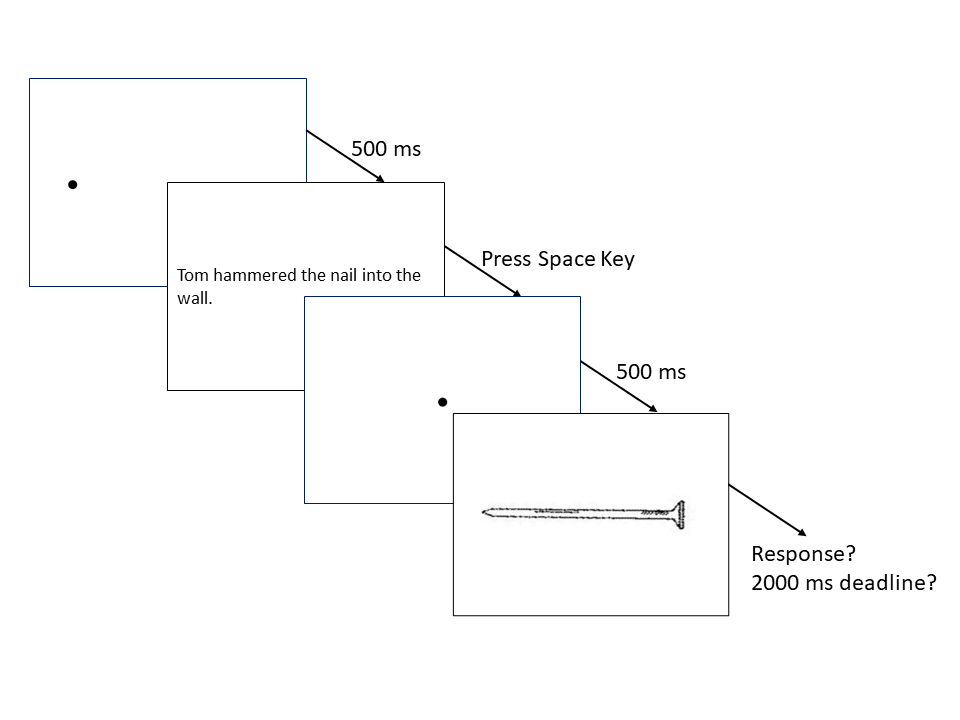
\includegraphics[width=1\linewidth]{includes/fig/fig2a} \caption{Procedure of the sentence-picture verification task, with an example of matching orientation.}\label{fig:fig01}
\end{figure}

Mental simulation effects have been demonstrated for object shape
(Zwaan et al., 2002), color
(Connell, 2007), and orientation
(Stanfield \& Zwaan, 2001). Subsequent replication studies revealed
consistent results for shape but inconsistent findings for color and
orientation effects (De Koning et al., 2017; Rommers et al., 2013; Zwaan \& Pecher, 2012). Existing theoretical frameworks
do not provide much guidance regarding the potential causes for this
discrepancy. With the accumulating concerns about the lack of
reproducibility (e.g., Kaschak \& Madden, 2021), researchers
have found it challenging to reconcile the theory of mental simulation
with the failures to replicate some of the effects (e.g, Morey et al., 2022). In
an empirical discipline like cognitive science, a theory requires the
support of reproducible results.

The reliability of match advantage effects seems to vary depending on
both the object properties and the languages under study. Mental
simulation effects for object shape have consistently been found in
English (Zwaan et al., 2017; Zwaan \& Madden, 2005; Zwaan \& Pecher, 2012), Chinese (Li \& Shang, 2017),
Dutch (De Koning et al., 2017; Engelen et al., 2011; Pecher et al., 2009; Rommers et al., 2013), German
(Koster et al., 2018), Croatian
(Šetić \& Domijan, 2017), and Japanese
(Sato et al., 2013). Object orientation, on the other hand, has
produced mixed results across languages: namely, positive evidence in
English (Stanfield \& Zwaan, 2001; Zwaan \& Pecher, 2012)
and in Chinese (Chen et al., 2020), and null evidence in Dutch
(De Koning et al., 2017; Rommers et al., 2013) and in German
as second language (Koster et al., 2018). Among studies on
shape and orientation, the effects of object orientation have been
smaller than those of object shape (e.g., \emph{d} = 0.10 vs.~0.17 in
Zwaan and Pecher (2012); \emph{d} = 0.07 vs.~0.27 in
De Koning et al. (2017)). To understand the causes for the discrepancies
among object properties and languages, it is imperative to consider the
cross-linguistic and experimental factors of the sentence-picture
verification task.

\hypertarget{cross-linguistic-methodological-and-cognitive-factors}{%
\subsection{Cross-linguistic, Methodological, and Cognitive Factors}\label{cross-linguistic-methodological-and-cognitive-factors}}

Several factors might contribute to cross-linguistic differences in the
match simulation effect of orientation. First, languages differ in how
they encode motion and placement events in sentences
(Newman, 2002; Verkerk, 2014). Second, the
potential role of mental rotation as a confound has been considered
(Rommers et al., 2013). We expand on how linguistic,
methodological, and cognitive factors hinder the improvement of
theoretical frameworks below.

\textbf{Linguistic Factors.} The probe sentences used in object orientation
studies usually contain several motion events (e.g., \emph{The ant walked
towards the pot of honey and tried to climb in}). Languages encode
motion events in different ways, and grammatical differences between
lexical encodings could explain different match advantage results.
According to Verkerk (2014), Germanic languages (e.g., Dutch, English, and
German) generally encode the manner of motion in the verb (e.g., \emph{The
ant dashed}), while conveying the path information through satellite
adjuncts (e.g., \emph{towards the pot of honey}). In contrast, other
languages, such as the Romance family (e.g., Portuguese, Spanish), more
often encode the path in the verb (e.g., \emph{crossing}, \emph{exiting}).
Crucially, past research on the match advantage of object orientation is
exclusively based on Germanic languages, and yet, there were differences
across those languages, with English being the only one that
consistently yielded the match advantage. As a minor difference across
Germanic languages in this regard, Verkerk (2014) notes that path-only
constructions (e.g., \emph{The ant went to the feast}) are more common in
English than in other Germanic languages.

Another topic to be considered is the lexical encoding of placement in
each language, as the stimuli contain several placement events (e.g.,
\emph{Sara situated the expensive plate on its holder on the shelf}).
Chen et al. (2020) and Koster et al. (2018) noted that
some Germanic languages, such as German and Dutch, often make the
orientation of objects more explicit than English. In English, for
example, the verb \emph{put} does not imply orientation in the sentences \emph{She
put the book on the table} and \emph{She put the bottle on the table.}
However, in German and Dutch, speakers preferred the verbs \emph{laid} or
\emph{stood} in the above sentences. In this case, the verb \emph{lay} encodes a
horizontal orientation, whereas the verb \emph{stand} encodes a vertical
orientation. This distinction extends to verbs indicating existence. As
Newman (2002) exemplified, an English
speaker would be likely to say \emph{There's a lamp in the corner,} whereas a
Dutch speaker would be more likely to say \emph{There `stands' a lamp in the
corner.} Nonetheless, we cannot conclude that these cross-linguistic
differences are affecting the match advantage across languages because
the current theories (e.g., Language and Situated Simulation, Barsalou, 2008) have not addressed the potential influence of
linguistic aspects such as the lexical encoding of events.

\textbf{Methodological factors.} Inconsistent findings on the match advantage
of object orientation may be due to variability in task design. For
example, studies failing to detect the match advantage may not have
required participants to verify the probe sentence after the response to
the target picture (see Zwaan, 2014a). Without such a
verification, participants might have paid less attention to the meaning
of the probe sentences, in which they would have been less likely to
form a mental representation of the objects (e.g., Zwaan \& van Oostendorp, 1993). In this regard, variability
originating from differences in the characteristics of experiments can
substantially influence the results
(Barsalou, 2019; Kaschak \& Madden, 2021).

\textbf{Cognitive Factors.} Since Stanfield and Zwaan (2001) showed a match
advantage of object orientation, later studies on this topic have
examined the association between the match advantage and alternative
cognitive mechanisms rather than situated simulation. One of these
potential mechanisms is spatial cognition, which can be measured with
mental rotation tasks. Indeed, studies have suggested that mental
rotation tasks offer valid reflections of previous spatial experience
(Frick \& Möhring, 2013) and of current spatial cognition
(Chu \& Kita, 2008; Pouw et al., 2014). Some
previous studies have drawn on mental rotation to study mental
simulation. For instance, De Koning et al. (2017) observed that the
effectiveness of mental rotation increased with the size of the depicted
object. Chen et al. (2020) examined the implication of this finding
for the match advantage of object orientation (Stanfield \& Zwaan, 2001),
and implemented a picture-picture verification task using the mental
rotation paradigm (D. Cohen \& Kubovy, 1993). In each trial, two
pictures appeared on opposite sides of the screen. Participants had to
verify whether the pictures represented identical or different objects.

This study not only revealed shorter verification times for matching
orientations (i.e., two identical pictures presented in horizontal or
vertical orientation) but also replicated the larger effect for larger
objects (i.e., pictures of bridges versus pictures of pens). The results
were consistent across the three languages investigated: English, Dutch
and Chinese. Compared to the results of sentence-picture verification
and picture-picture verification, Chen et al. (2020) converted the
picture-picture verification times to the mental rotation scores that
were the discrepancy of verification times between the identical and
different orientations\footnote{In the pre-registered plan, we used the term ``imagery score'' but
  this term was confusing. Therefore, we used ``mental rotation scores''
  instead of ``imagery scores'' in the final report.}. Their analysis showed that mental rotation
affected the Dutch participants' sentence-picture verification
performance. With the measurement of mental rotation scores, we explore
the association of spatial cognition and the effect of orientation in
comprehension across the investigated languages.

\hypertarget{purposes-of-this-study}{%
\subsection{Purposes of this study}\label{purposes-of-this-study}}

To scrutinize the discrepancies in findings across languages and
cognitive factors, we examined the reproducibility of the object
orientation effect in a multi-lab collaboration. Our pre-registered plan
aimed at detecting a general match advantage of object orientation
across languages and evaluated the magnitude of match advantage in each
specific language. Additionally, we examined whether the match
advantages were related to the mental rotation index. Thus, this study
followed the original methods from (Stanfield \& Zwaan, 2001) and
addressed two primary questions: (1) How much of the match advantage of
object orientation can be obtained within different languages, and (2)
How do differences in the mental rotation index affect the match
advantage across languages?

\hypertarget{method}{%
\section{Method}\label{method}}

\hypertarget{hypotheses-and-design}{%
\subsection{Hypotheses and Design}\label{hypotheses-and-design}}

The study design for the sentence-picture and picture-picture
verification tasks was mixed, using between-participant (language) and
within-participant (match versus mismatch object orientation)
independent variables. In the sentence-picture verification task, the
match condition reflects a match between the sentence and the picture,
whereas in the picture-picture verification it reflects a match in
orientation between two pictures. The only dependent variable for both
tasks was response time. The time difference between conditions in each
task is the measurement of mental simulation effects (for the
sentence-picture task) and mental rotation scores (for the
picture-picture task). We did not select languages systematically, but
instead based on our collaboration recruitment with the Psychological
Science Accelerator (PSA, Moshontz et al., 2018).

We pre-registered the following hypotheses:

\begin{enumerate}
\def\labelenumi{(\arabic{enumi})}
\item
  In the sentence-picture verification task, we expected response
  times to be shorter for matching compared to mismatching
  orientations within each language. In the picture-picture
  verification task, we expected shorter response time for identical
  orientation compared to different orientations. We did not have any
  specific hypotheses about the relative size of the object
  orientation match advantage in different languages.
\item
  Based on the assumption that `mental rotation is a general cognitive
  function', we expect equal mental rotation scores across languages,
  but no association between mental rotation scores and mental
  simulation effects (see Chen et al., 2020).
\end{enumerate}

\hypertarget{participants}{%
\subsection{Participants}\label{participants}}

The pre-registered power analysis indicated the need to include \emph{n} =
156 and 620 participants for 80\% power for a directional one-sample
\emph{t}-test for a \emph{d} = 0.20 and 0.10, respectively. A mixed-model
simulation suggested that \emph{n} = 400 participants with 100 items (i.e.,
24 planned items nested within at least five languages) would produce
90\% power to detect the same effect as that reported in
Zwaan and Pecher (2012). The laboratories were allowed to
follow a secondary plan: a team collected at least their pre-registered
minimum sample size (suggested 100 to 160 participants, most implemented
50), and then determine whether or not to continue data collection via
Bayesian sequential analysis (stopping data collection if \(BF_{10}\) = 10
or 0.10)\footnote{See details of power analysis in the pre-registered plan, pp.~13 -
  15. \url{https://psyarxiv.com/t2pjv/}}.

We collected data in 18 languages from
50 laboratories. Each
laboratory chose a maximal sample size and an incremental \emph{n} for
sequential analysis before their data collection. Because the
pre-registered power analysis did not match the final analysis plan, we
additionally completed a sensitivity analysis to ensure the sample size
was adequate to detect small effects, and the results indicated that if
the observe orientation difference in reaction time between the
different orientations was overall 2.36 ms or higher, the effect would
be detected as significant. Appendix A summarizes the details of the
sensitivity analysis.

The original sample sizes are presented in Table \ref{tab:sample-table}
for the teams that provided raw data to the project. Data collection
proceeded in two broad stages: initially we collected data in the
laboratory. However, when the global COVID-19 pandemic made this
practice impossible to continue, we moved data collection online. In
total,
4,248
unique participants completed the present study with
2,843
completing the in-person version and
1,405
completing the online version\footnote{Data for this study was collected together with another unrelated
  study (Phills et al., 2022) during the same data collection
  session, with the two studies using different data collection
  platforms. The demographic data was collected within the platform of
  the other study during the in-person sessions. Some participants
  only completed the Phills et al.~study and dropped out without
  completing the present study, and there were also some data entry
  errors in the demographic data. Thus, the demographic data of some
  participants who took the present study are missing or
  unidentifiable (\emph{n} =
  39
  cannot be matched to a lab, \emph{n} =
  2,053
  were missing gender information, and \emph{n} =
  332 were missing age
  information). Importantly, this does not affect the integrity of the
  experimental research data.}. The in-person version included
35
research teams and the online version included
19
with 50 total teams across both data
collection methods (i.e., some labs completed both in-person and online
data collection). Based on recommendations from the research teams
(TUR\_007, TWN\_002), two sets of data were excluded from all analyses due
to participants being non-native speakers. Figure \ref{fig:sample-fig}
provides a flow chart for participant exclusion and inclusion for
analyses. All participating laboratories had either ethical approval or
institutional evaluation before data collection. All data and analysis
scripts are available on the source files
(\url{https://codeocean.com/capsule/3994879}). Appendix B summarizes the
average characteristics by language and laboratory.

\begin{table}[tbp]

\begin{center}
\begin{threeparttable}

\caption{\label{tab:sample-table}Demographic and Sample Size Characteristics}

\footnotesize{

\begin{tabular}{lccccccccc}
\toprule
Language & $SP_{Trials}$ & $PP_{Trials}$ & $SP_N$ & $PP_N$ & $Demo_N$ & $Female_N$ & $Male_N$ & $M_{Age}$ & $SD_{Age}$\\
\midrule
Arabic & 2544 & 2544 & 106 & 106 & 107 & 42 & 12 & 32.26 & 18.59\\
Brazilian Portuguese & 1200 & 1200 & 50 & 50 & 50 & 36 & 13 & 30.80 & 8.73\\
English & 45189 & 45312 & 1884 & 1888 & 2055 & 1360 & 465 & 21.71 & 3.85\\
German & 5616 & 5616 & 234 & 234 & 248 & 98 & 26 & 22.34 & 3.40\\
Greek & 2376 & 2376 & 99 & 99 & 109 & 0 & 0 & 33.86 & 11.30\\
Hebrew & 3576 & 3571 & 149 & 149 & 181 & 0 & 0 & 24.25 & 9.29\\
Hindi & 1896 & 1896 & 79 & 79 & 86 & 57 & 27 & 21.66 & 3.46\\
Magyar & 3610 & 3816 & 151 & 159 & 168 & 3 & 1 & 21.50 & 2.82\\
Norwegian & 3576 & 3576 & 149 & 149 & 154 & 13 & 9 & 25.22 & 6.40\\
Polish & 1368 & 1368 & 57 & 57 & 146 & 0 & 0 & 23.25 & 7.96\\
Portuguese & 1488 & 1464 & 62 & 61 & 55 & 26 & 23 & 30.74 & 9.09\\
Serbian & 3120 & 3120 & 130 & 130 & 130 & 108 & 21 & 21.38 & 4.50\\
Simplified Chinese & 2040 & 2016 & 85 & 84 & 96 & 0 & 1 & 21.92 & 4.68\\
Slovak & 3881 & 3599 & 162 & 150 & 325 & 1 & 0 & 21.77 & 2.33\\
Spanish & 3120 & 3096 & 130 & 129 & 146 & 0 & 0 & 21.73 & 3.83\\
Thai & 1200 & 1152 & 50 & 48 & 50 & 29 & 9 & 21.54 & 3.81\\
Traditional Chinese & 3600 & 3600 & 150 & 150 & 186 & 69 & 46 & 20.89 & 2.44\\
Turkish & 6456 & 6432 & 269 & 268 & 274 & 36 & 14 & 21.38 & 4.59\\
\bottomrule
\addlinespace
\end{tabular}

}

\begin{tablenotes}[para]
\normalsize{\textit{Note.} SP = Sentence Picture Verification, PP = Picture Picture Verification. Sample sizes for demographics may be higher than the sample size for the this study, as participants could have only completed the bundled experiment. Additionally, not all entries could be unambigously matched by lab ID, and therefore, demographic sample sizes could also be less than data collected.}
\end{tablenotes}

\end{threeparttable}
\end{center}

\end{table}

\begin{figure}
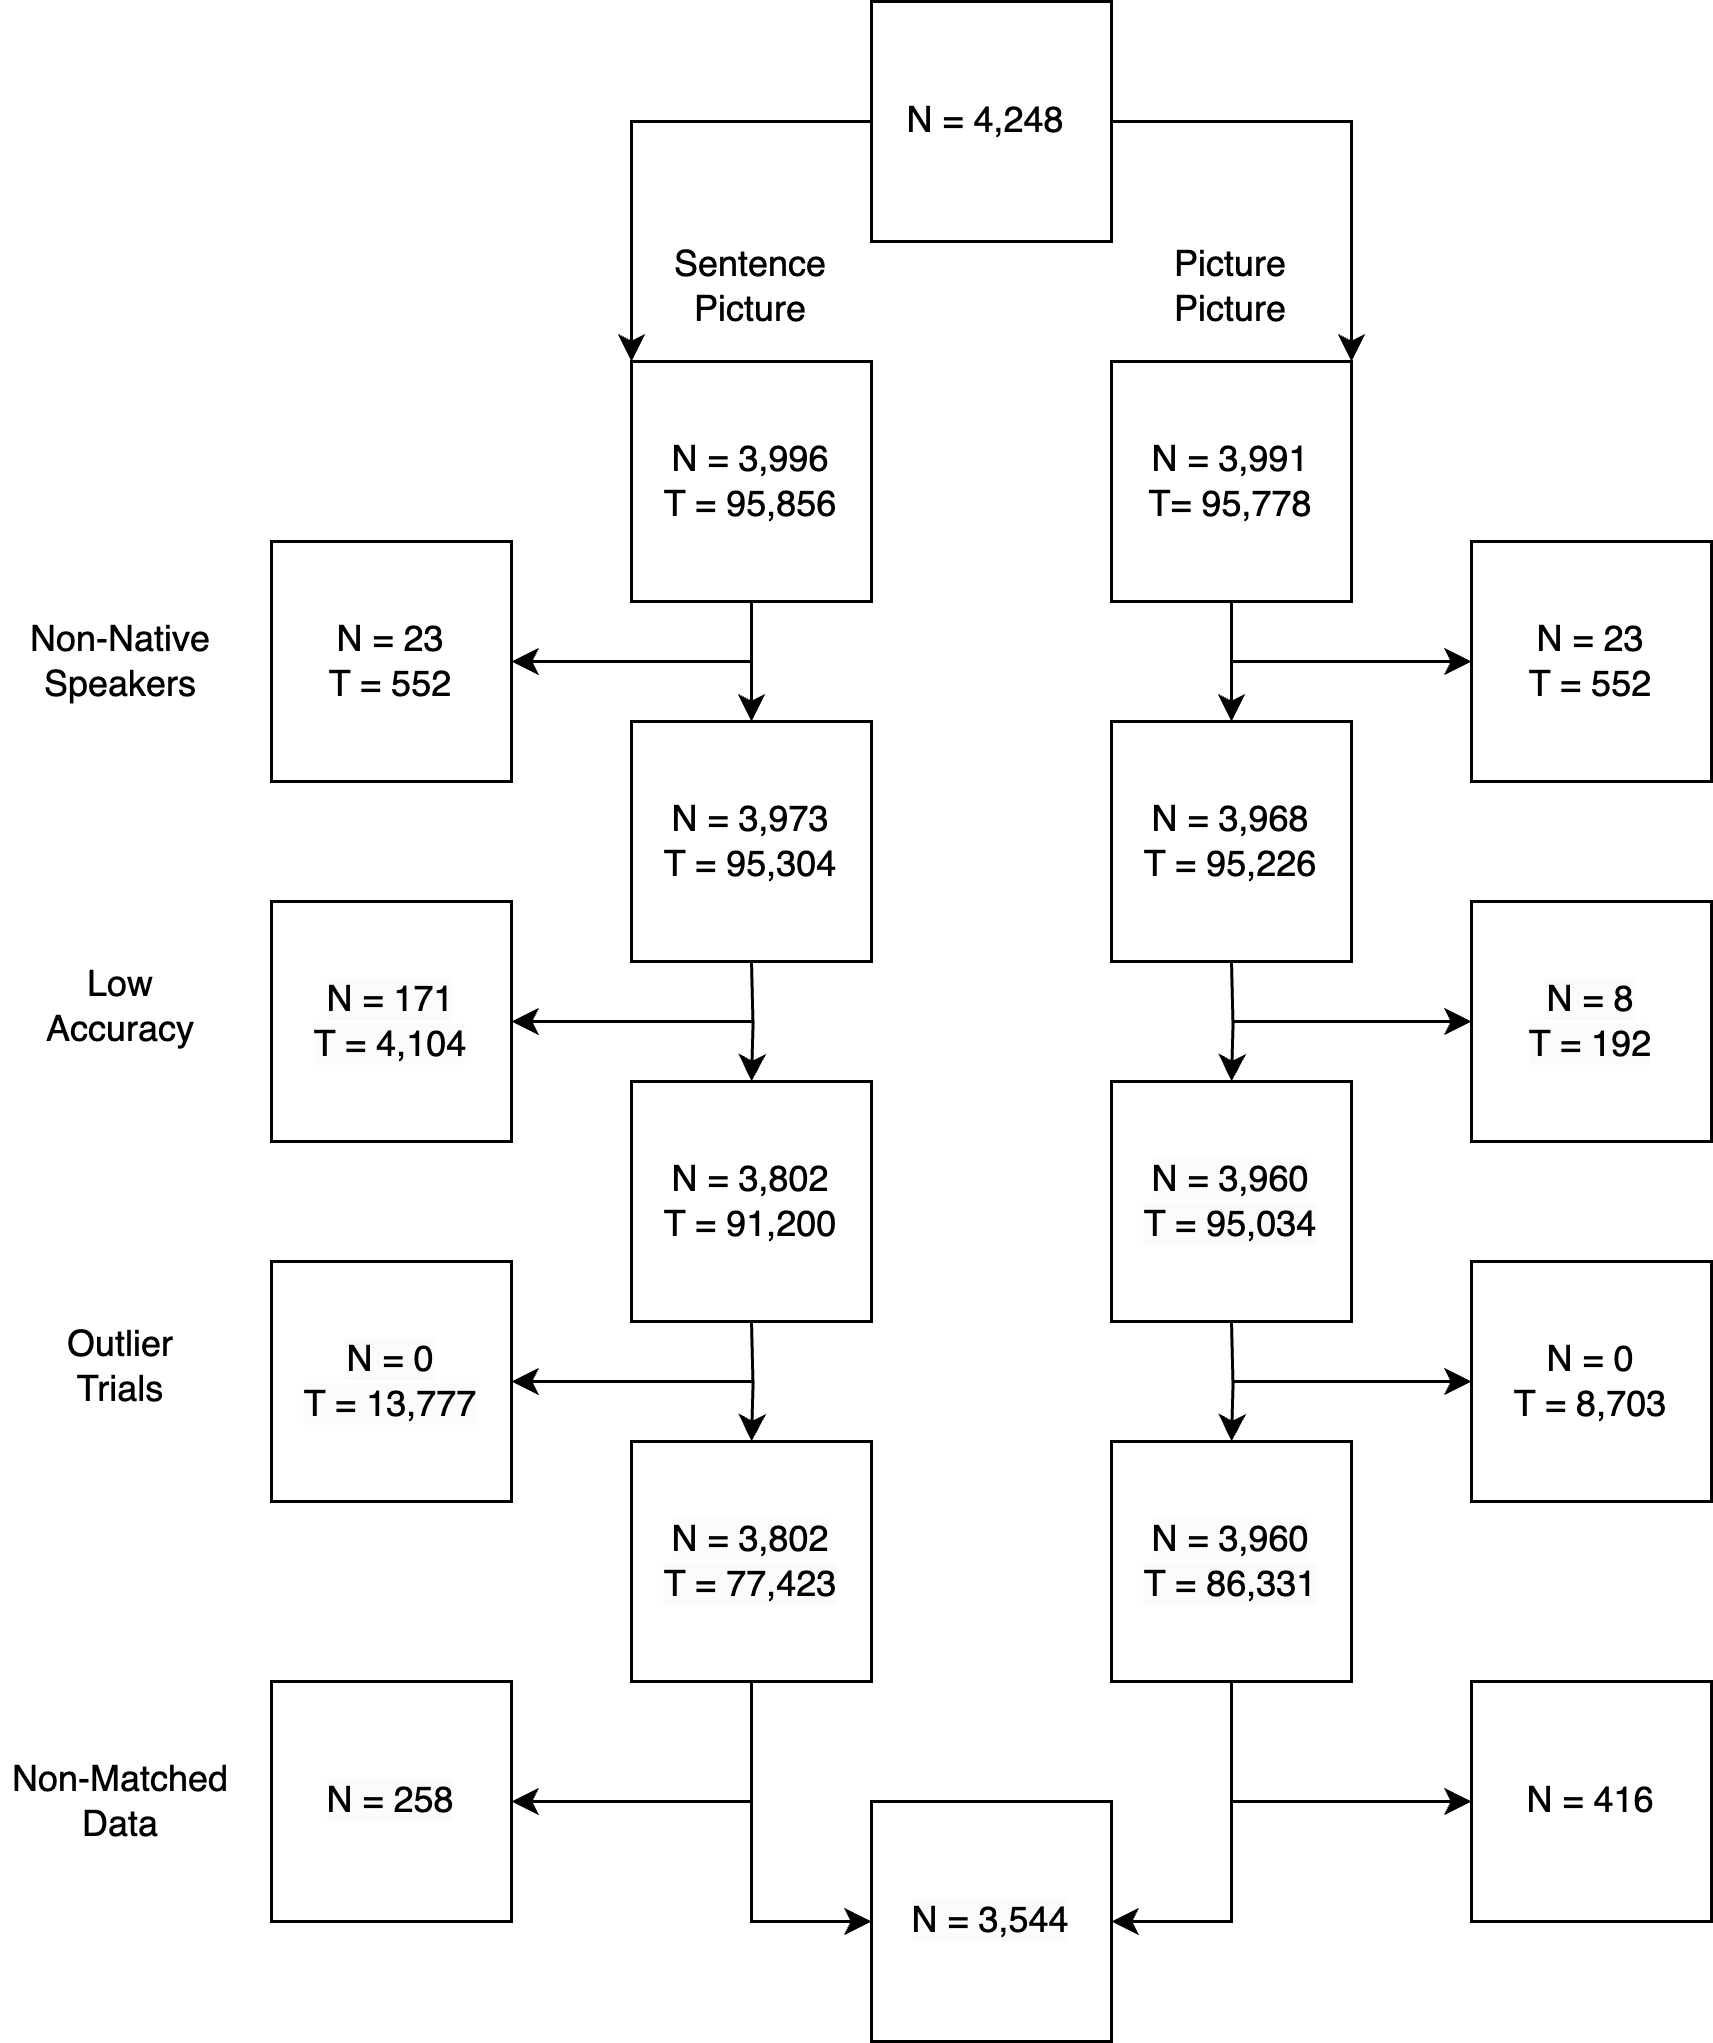
\includegraphics[width=5.71in]{includes/fig/psa002_flow.drawio} \caption{Sample size and exclusions. N = number of unique participants, T = number of trials. The final combined sample was summarized to a median score for each match/mismatch condition, and therefore, includes one summary score per person.}\label{fig:sample-fig}
\end{figure}

\hypertarget{materials}{%
\subsection{Materials}\label{materials}}

\textbf{Sentences.} 24 critical sentence pairs (48 total sentences) were
included in this study following Stanfield and Zwaan (2001). Each pair
consisted of versions that differed in their implied orientation of the
object embedded in the sentence. For instance, the sentence \emph{The
librarian put the book back on the table} - which implies a horizontal
orientation - had a counterpart in the sentence \emph{The librarian put the
book back on the shelf} - which implies a vertical orientation. Another
two sets of 24 sentences were included as filler sentences for the task,
and each participant received only one set of these two randomized
versions. These were not matched to any particular orientation but
included a potential object for depiction. For example, \emph{After a week
the painting arrived by mail}, and \emph{The flowers that were planted last
week had survived the storm} were included as filler sentences. Each
participant was shown 24 critical sentences and 24 filler sentences in
the study. The filler sentences were included to counterbalance the
number of yes-no answers to create an even 50\% ratio.

\textbf{Pictures.} The study included 24 critical matched pictures that only
varied in their orientation (vertical/horizontal) for a total of 48
critical pictures. These pictures were matched to their respective
sentences for implied orientation. \emph{The librarian put the book back on
the table} was matched with a horizontally-oriented book, while \emph{The
librarian put the book back on the shelf} was matched with a
vertically-oriented book. For counterbalancing, the mismatch between
picture orientation and sentence was created, and the book would be
shown in the respective opposite orientation (see orientation pairs at
\url{https://osf.io/utqxb}). Another 48 pictures were included for the
fillers which were unrelated to the corresponding sentence. Therefore,
the answer to critical pairs was always ``yes'', while the filler
sentence-picture combinations answer was always ``no''.

\textbf{Picture-Picture Trials.} The picture-picture verification task used
the same object pictures as the above task. The 24 critical picture
pairs were included as match trials and were counterbalanced such as
half the time they appeared with the same object and orientation (i.e.,
the same picture), and half the time with the opposite orientation
(i.e., horizontal and vertical). The filler pictures were randomly
paired to create mismatch trials. Table \ref{tab:stim-table} shows the
counterbalancing and combinations for trials.

\begin{table}[tbp]

\begin{center}
\begin{threeparttable}

\caption{\label{tab:stim-table}Trial conditions for the Sentence-Picture and Picture-Picture Verification Task}

\scriptsize{

\begin{tabular}{lllcc}
\toprule
Condition & Item 1 & Item 2 & Answer & Number\\
\midrule
Sentence-Picture
Critical
Match & Critical Sentence:
Horizontal & Critical Picture:
Horizontal & Yes & 6\\
Sentence-Picture
Critical
Match & Critical Sentence:
Vertical & Critical Picture:
Vertical & Yes & 6\\
Sentence-Picture
Critical
Mismatch & Critical Sentence:
Horizontal & Critical Picture:
Vertical & Yes & 6\\
Sentence-Picture
Critical
Mismatch & Critical Sentence:
Vertical & Critical Picture:
Horizontal & Yes & 6\\
Sentence-Picture
Filler & Sentence & Picture & No & 24\\
Picture-Picture
Critical
Match & Critical Picture:
Horizontal & Critical Picture:
Horizontal & Yes & 6\\
Picture-Picture
Critical
Match & Critical Picture:
Vertical & Critical Picture:
Vertical & Yes & 6\\
Picture-Picture
Critical
Mismatch & Critical Picture:
Horizontal & Critical Picture:
Vertical & Yes & 6\\
Picture-Picture
Critical
Mismatch & Critical Picture:
Vertical & Critical Picture:
Horizontal & Yes & 6\\
Picture-Picture
Filler & Picture & Picture & No & 24\\
\bottomrule
\end{tabular}

}

\end{threeparttable}
\end{center}

\end{table}

\hypertarget{procedure}{%
\subsection{Procedure}\label{procedure}}

\textbf{Sentence-Picture Task.} The sentence-picture verification task was
always administered first. This task began with six practice trials.
Each trial started with a left-aligned vertically-centered fixation
point displayed for 1,000 ms, immediately followed by the probe
sentence. The sentence remained on the screen until the participant
pressed the space key, acknowledging that they had read the sentence.
Then, the object picture (from Zwaan \& Pecher, 2012) was
presented in the center of the screen until the participant responded,
or it disappeared after two seconds. Participants were instructed to
verify, as quickly and accurately as possible, whether the object on
screen had been mentioned in the probe sentence. Following
Stanfield and Zwaan (2001), a memory check test was carried out after every
three to eight trials to ensure that participants had read each sentence
carefully.

As shown in Table \ref{tab:stim-table}, the trials for the
sentence-picture task were created by counterbalancing the sentence
implied orientation (vertical, horizontal) by the pictured object
orientation creating a fully-crossed combination between matching
sentences and objects. Therefore, each participant only saw one of the
four possible combinations (sentence orientation 2 x object orientation
2). For the filler items, sentences and pictures were randomly assigned
in two separate patterns, and these were included with the critical
pairs. Stimuli lists were created in Excel, and this information can be
found at \url{https://osf.io/utqxb}.

\textbf{Translation of Sentences.} The translation of probe sentences
followed our pre-registered plan. Every non-English language coordinator
was required to recruit at least four translators who were fluent in
both English and the target language. Every language coordinator
supervised the translators using the Psychological Science Accelerator
guidelines (\url{https://psysciacc.org/translation-process/}). In addition,
the coordinator and participating laboratories consulted about each of
the following points:

\begin{enumerate}
\def\labelenumi{\arabic{enumi})}
\item
  Four translators could denote the items that are unfamiliar to a
  particular language based on object familiarity ratings. The two
  forward translators would suggest alternative probe sentences and
  object pictures to replace the unfamiliar objects. The two backward
  translators would evaluate the suggested items.
\item
  Some objects in a particular language have different spellings or
  pronunciations among countries and geographical zones due to
  dialect. For example, American speakers tend to write \emph{tire} whereas
  British speakers tend to write \emph{tyre.} Every coordinator would mark
  these local translations in the final version of translated
  materials. Participating laboratories could replace the names to
  match the local dialect.
\end{enumerate}

\textbf{Picture-Picture Task.} Next, the picture-picture verification task
was administered. In each trial, two objects appeared on either side of
the central fixation point until either the participant indicated that
the pictures displayed the same object or two different objects, or
until two seconds elapsed. As shown in Table \ref{tab:stim-table}, four
possible combinations of critical orientations could be shown with the
picture (same, different) by orientation (same, different). Each
participant only saw one of the critical combinations, and filler items
were randomly paired in two combinations to match. The stimuli lists can
be found at \url{https://osf.io/utqxb}.

\textbf{Software Implementation.} The study was executed using OpenSesame
software for millisecond timing
(Mathôt et al., 2012). After data collection moved
online, to minimize the differences between on-site and web-based
studies, we converted the original Python code to Javascript and
collected the data using OpenSesame through a JATOS server
(Lange et al., 2015; Mathôt \& March, 2022). We proceeded with
the online study from February to June 2021 after the changes in the
procedure were approved by the journal editor and reviewers. Following
the literature, we did not anticipate any theoretically important
differences between the two data collection methods (see Anwyl-Irvine et al., 2020; Bridges et al., 2020; de Leeuw \& Motz, 2016). The instructions and experimental
scripts are available at the public OSF folder (\url{https://osf.io/e428p/}
``Materials'' in Files).

\hypertarget{analysis-plan}{%
\subsection{Analysis Plan}\label{analysis-plan}}

To test hypothesis 1, our first planned analysis\footnote{See the analysis plan in the pre-registered plan, pp.~19 - 20,
  \url{https://psyarxiv.com/t2pjv/}. This plan was changed to a
  random-effects model to ensure that we did not assume the exact same
  effect size for each language and lab.} used a
random-effects meta-analysis model that estimated the match advantage
across laboratories and languages. The meta-analysis summarized the
median reaction times by match condition to determine the effect size by
laboratory. The following formula was used:

\[d = \frac{Mdn_{Mismatch} - Mdn_{Match}}{\sqrt{MAD_{Mismatch}^2 + MAD_{Match}^2-2\times r\times MAD_{Mismatch} \times MAD_{Match}}} \times \sqrt{2 \times (1-r)}\]

where \(d\) is Cohen's \(d\) (Fritz et al., 2012), \(Mdn\) is Median, \(MAD\) is median
absolute deviation, and \(r\) is correlation between match and mismatch
condition. Meta-analytic effect sizes were computed for those languages
that had data from more than one team.

Continuing to test hypothesis 1, next, we ran planned mixed-effects
models using each individual response time from the sentence-picture
verification task as the dependent variable. In each analysis, we first
built a simple linear regression model with a fixed intercept only.
Then, we systematically added random intercepts and fixed effects,
arriving at the final model. First, the random intercepts were added to
the model one-by-one in the following order: participant ID, target,
laboratory ID, and finally language. Please see below for decision
criteria for determining the final random-effect structure. Then, the
fixed effect of matching condition (match vs.~mismatch) was added to the
model. Language-specific mixed-effects models were conducted in the same
way if the meta-analysis showed a significant orientation effect.

According to the pre-registration, we planned to test hypothesis 2 by
first evaluating the equality of mental rotation scores across languages
using an ANOVA. However, this plan was updated to use mixed models
instead due to the nested structure of the data (Gelman, 2006). The same
analysis plan was used for model building and selection as described
above for the sentence-picture verification task.

To further assess hypothesis 2, the last planned analysis was to use
mental rotation scores for the prediction of mental stimulation with an
interaction between language and mental rotation scores computed from
the picture-picture task to determine if there were differences in
prediction of match advantage in the sentence-picture task. Here, we
used a mixed-effects model as well to control for the random effect of
the data collection lab, and with language, mental rotation score, and
their interaction as fixed effect predictors.

\textbf{Decision criterion for model selection and hypothesis testing.} The
inclusion of both random and fixed effects in models was assessed using
model comparison based on the Akaike information criterion (AIC). While
this method is less conservative than alternatives such as the
likelihood ratio test (Matuschek et al., 2017), the AIC was deemed appropriate
due to the modest effect sizes that tend to be produced by mental
simulation effects, and the limited sample sizes in the present study
(albeit larger samples than those of most previous studies). Models with
lower AIC were preferred over models with higher AIC, and in cases where
the difference in AIC did not reach 2 (Burnham \& Anderson, 1998), the model with
fewer parameters was preferred.

\emph{p}-values for each effect were calculated using the Satterthwaite
approximation for degrees of freedom for individual predictor
coefficients and meta-analysis (Luke, 2017).
\emph{p}-values were interpreted using the pre-registered \(\alpha\) level of
.05.

\textbf{Intra-lab analysis during data collection.}

Before data collection, each lab decided whether they wanted to apply a
sequential analysis (Schönbrodt et al., 2017) or
whether they wanted to settle for a fixed sample size. The
pre-registered protocol for labs applying sequential analysis
established that they could stop data collection upon reaching the
pre-registered criterion (\(BF_{10}\) = 10 or .10), or the maximal sample
size. Each laboratory chose a fixed sample size and an incremental n for
sequential analysis before their data collection. Two laboratories
(HUN\_001, TWN\_001) stopped data collection at the pre-registered
criterion, \(BF_{10}\) = .10. Fourteen laboratories did not finish the
sequential analysis because (1) twelve laboratories were interrupted by
the pandemic outbreak; (2) two laboratories (TUR\_007E, TWN\_002E)
recruited English-speaking participants to comply with institutional
policies. Lab-based records were reported on a public website as each
laboratory completed data collection (details are available in Appendix
C).

\hypertarget{results}{%
\section{Results}\label{results}}

\hypertarget{data-screening}{%
\subsection{Data Screening}\label{data-screening}}

As shown in Figure \ref{fig:sample-fig}, participants' data were
deleted listwise from the sentence-picture and picture-picture tasks if
they did not perform with at least 70\% accuracy. Next, the data were
screened for outliers. Our pre-registered plan excluded outliers based
on a linear mixed-model analysis for participants in the third quantile
of the grand intercept (i.e., participants with the longest average
response times). After examining the data from both online and in-person
data collection, it became clear that both a minimum response latency
and maximum response latency should be employed, as improbable times
existed at both ends of the distribution. The minimum response time was
set to 160 ms based on Hick's Law (Kvålseth, 2021; Proctor \& Schneider, 2018). The maximum response latency was calculated
as two times the mean absolute deviation plus the median calculated
separately for each participant. Exclusions were performed at the trial
level for these outlier response times.

To ensure equivalence between data collection methods, we evaluated the
response times predicted by the fixed effects of the interaction between
match (match vs.~mismatch) and data collection source (in-person vs.
online). We included random intercepts for participants, lab, language,
and random slopes for source by lab and source by language. This
analysis showed no difference between data sources: \emph{b} =
2.41,
\emph{SE} =
2.77,
\emph{t}(73729.28)
=
0.87,
\emph{p} = .385. Therefore, the
following analyses did not separate in-person and online data. Table
\ref{tab:summary-languages} provides a summary of the match advantage
by language for the sentence-picture verification task.

Although we combined the two data sets in the final data analysis, it is
worth considering that online participants' attention may be easily
distracted given the lack of environmental control and experimenter
overview. However, this secondary task revealed that online participants
had a higher percent correct than in-person participants,
\emph{t}(3,214.86) = 35.77, \emph{p}
\textless{} .001, \(M_{online}\) =
85.46
(\emph{SD} =
14.20)
and \(M_{in-person}\) =
67.71
(\emph{SD} =
16.26).

\begin{table}[tbp]

\begin{center}
\begin{threeparttable}

\caption{\label{tab:summary-languages}Descriptive Summary of Sentence-Picture Verification Task by Language}

\begin{tabular}{lcccc}
\toprule
Language & Accuracy Percent & Mismatching & Matching & Match Advantage\\
\midrule
Arabic & 90.65 & 580.25 (167.53) & 581.00 (200.89) & -0.75\\
Brazilian Portuguese & 94.87 & 641.00 (136.40) & 654.50 (146.78) & -13.50\\
English & 95.04 & 576.75 (124.17) & 578.75 (127.87) & -2.00\\
German & 96.53 & 593.00 (106.75) & 576.00 (107.12) & 17.00\\
Greek & 92.35 & 753.50 (225.36) & 728.50 (230.91) & 25.00\\
Hebrew & 96.73 & 569.50 (98.59) & 574.50 (110.45) & -5.00\\
Hindi & 91.32 & 638.50 (207.19) & 662.00 (228.32) & -23.50\\
Hungarian & 96.47 & 623.00 (111.94) & 643.00 (129.73) & -20.00\\
Norwegian & 96.93 & 592.50 (126.39) & 612.00 (136.03) & -19.50\\
Polish & 96.11 & 601.00 (139.36) & 586.00 (108.23) & 15.00\\
Portuguese & 95.01 & 616.50 (144.55) & 607.00 (145.29) & 9.50\\
Serbian & 94.78 & 617.75 (158.64) & 635.00 (168.28) & -17.25\\
Simplified Chinese & 92.39 & 655.00 (170.50) & 642.50 (158.64) & 12.50\\
Slovak & 96.45 & 610.50 (125.28) & 607.25 (117.87) & 3.25\\
Spanish & 94.32 & 663.00 (147.52) & 676.00 (154.19) & -13.00\\
Thai & 93.92 & 652.50 (177.91) & 637.75 (130.10) & 14.75\\
Traditional Chinese & 94.41 & 625.00 (139.36) & 620.00 (123.06) & 5.00\\
Turkish & 95.38 & 654.50 (146.04) & 637.00 (126.02) & 17.50\\
\bottomrule
\addlinespace
\end{tabular}

\begin{tablenotes}[para]
\normalsize{\textit{Note.} Average accuracy percentage, Median response times and median absolute deviations (in parentheses) per match condition (Mismatching, Matching); Match advantage (difference in response times).}
\end{tablenotes}

\end{threeparttable}
\end{center}

\end{table}

\hypertarget{hypothesis-1-meta-analysis-of-the-orientation-effect}{%
\subsection{Hypothesis 1: Meta-Analysis of the Orientation Effect}\label{hypothesis-1-meta-analysis-of-the-orientation-effect}}

\begin{figure}
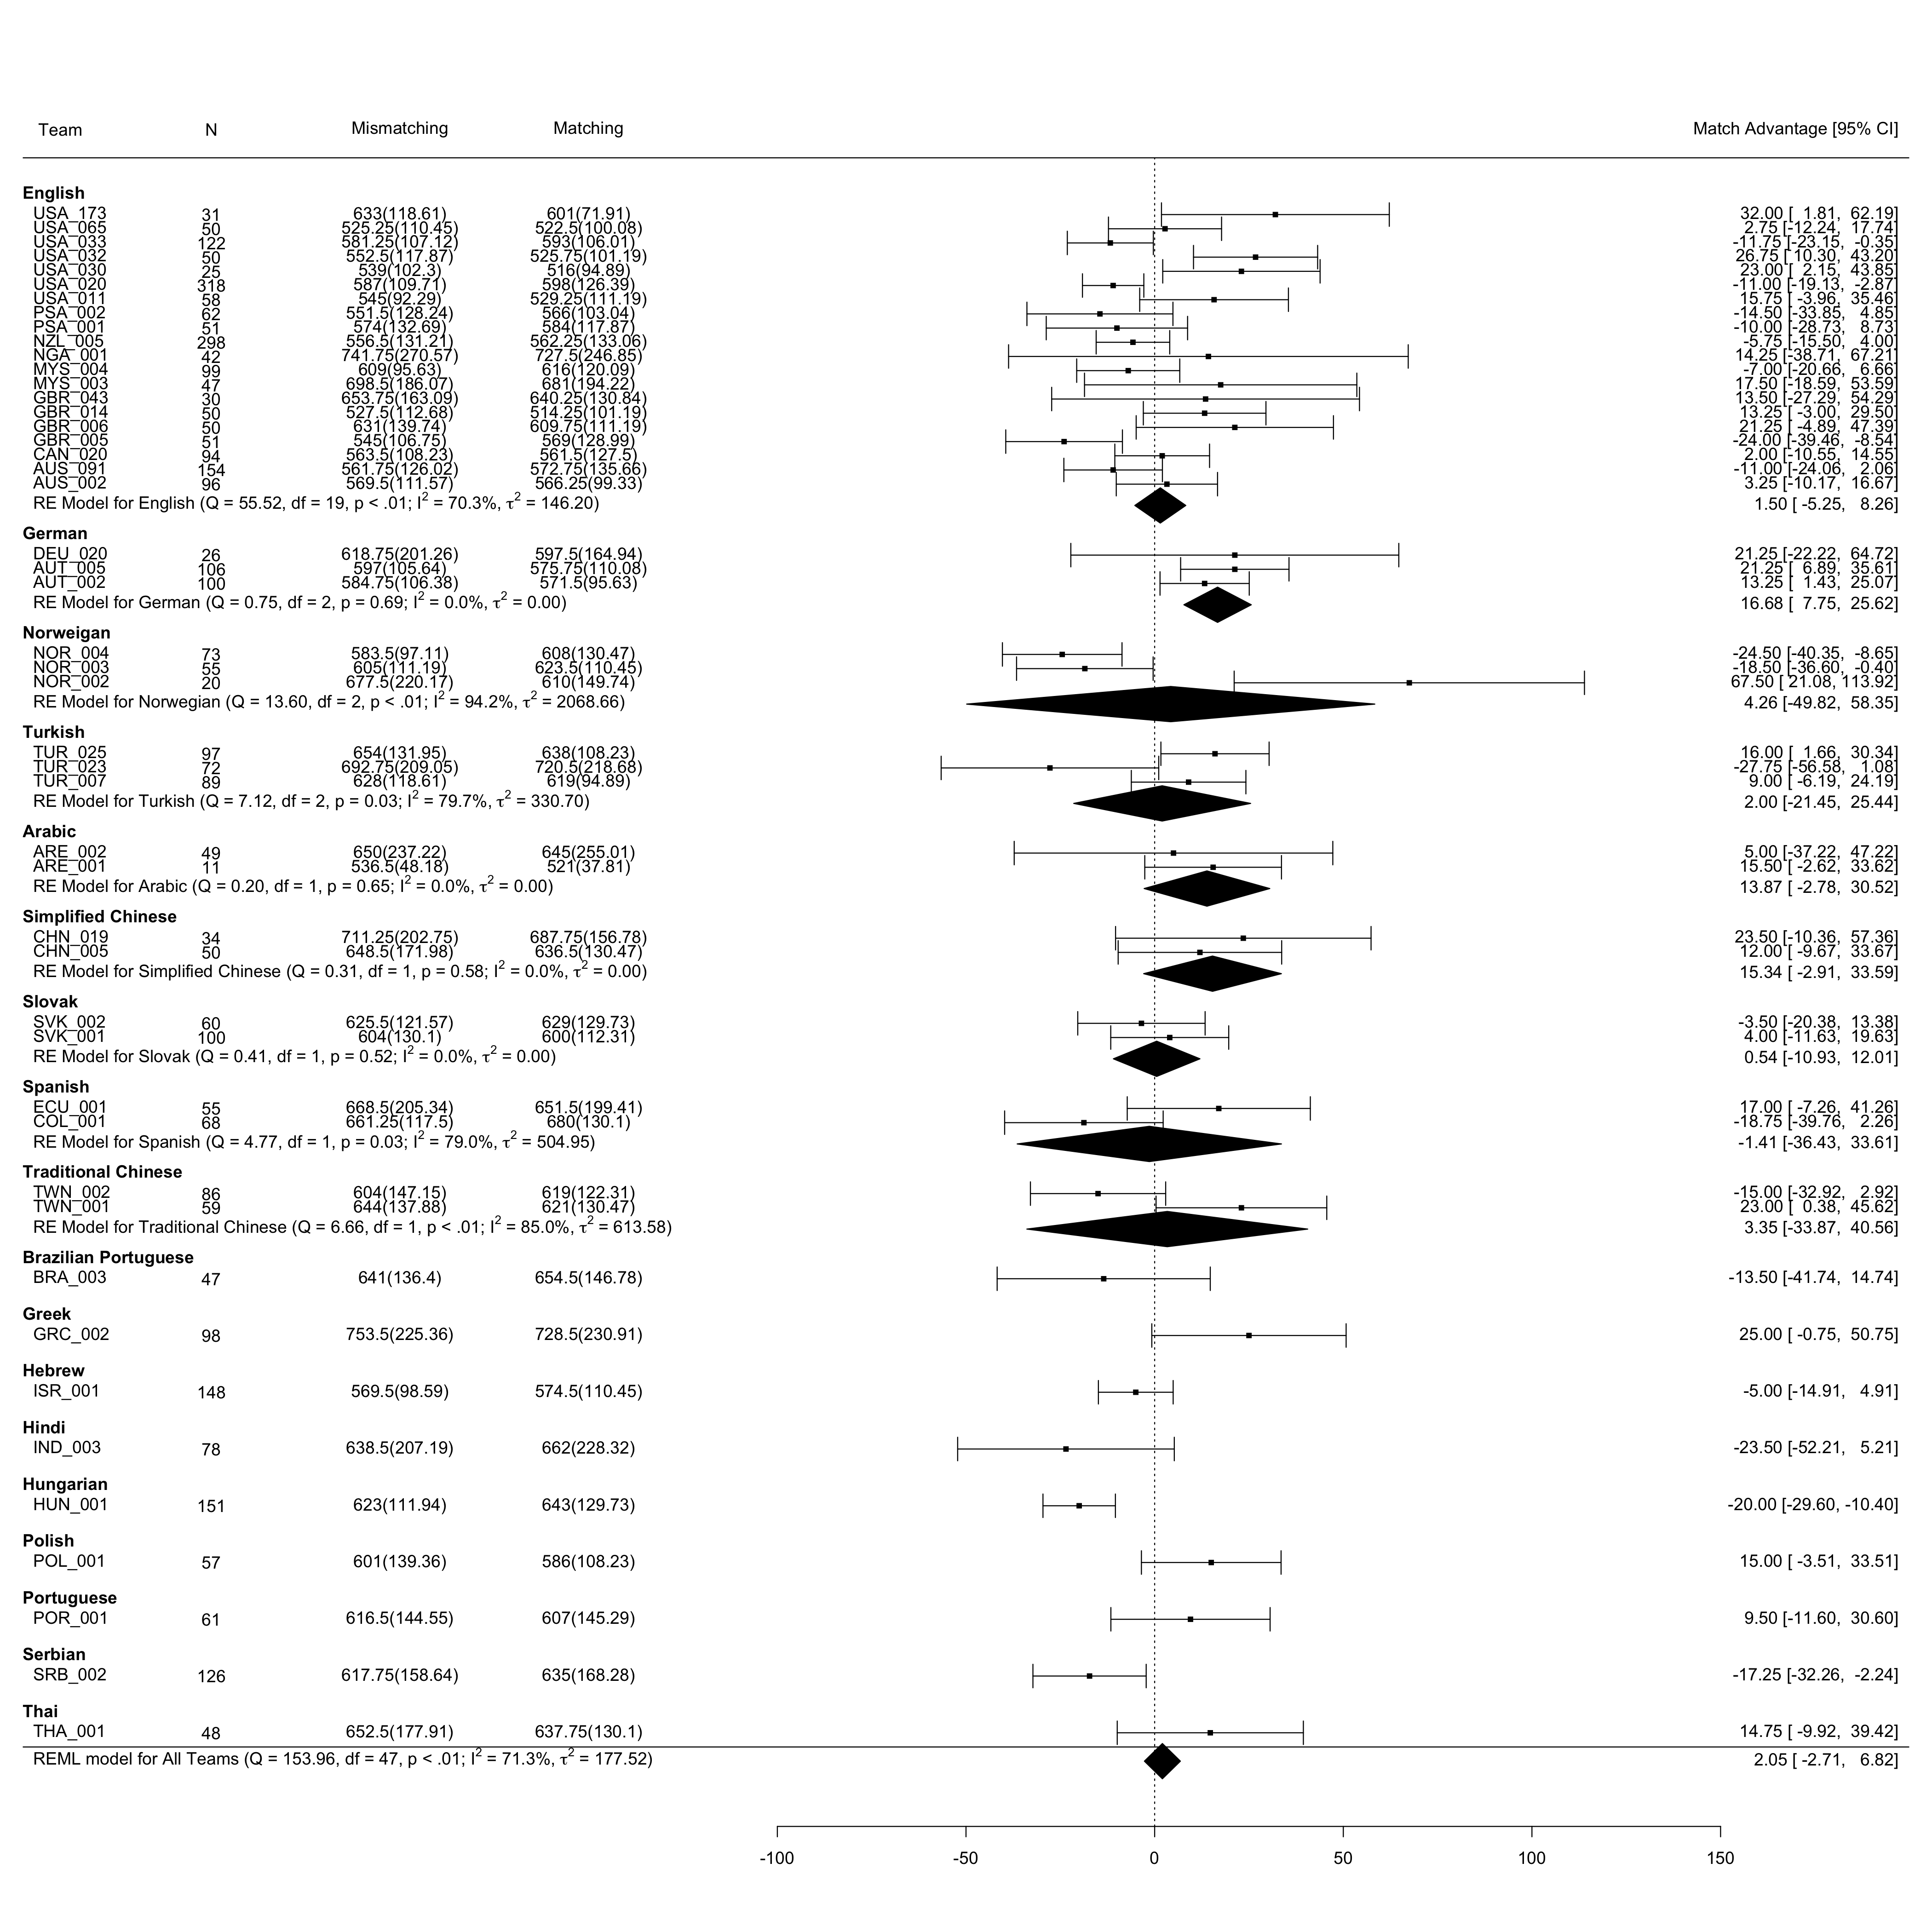
\includegraphics[width=1\linewidth,height=0.9\textheight]{includes/fig/meta-all} \caption{Meta-analysis on match advantage of object orientation for all languages. Diamonds indicate summary estimates, the midpoint of the diamond indicating the point estimate, and the left and right endpoints indicating the lower and upper bounds of the confidence interval of the estimated effect size. The lowermost diamond represents the estimate derived from the whole dataset.}\label{fig:meta-all-plot}
\end{figure}

The planned meta-analysis examined the effect overall and within
languages wherein at least two laboratories had collected data (Arabic,
English, German, Norway, Simplified Chinese, Traditional Chinese,
Slovakian, and Turkey). Figure \ref{fig:meta-all-plot} showed a
significant positive orientation effect across German laboratories (\emph{b}
= 16.68, 95\% CI
{[}7.75,
25.62{]}) but did not reveal a
significant overall effect (\emph{b} =
2.05, 95\% CI
{[}-2.71,
6.82{]}). Also, a significant
negative orientation effect was found in the Hungarian (\emph{b} = -20.00,
95\% CI {[}-29.60, -10.40{]}) and the Serbian laboratory (\emph{b} = -17.25, 95\%
CI {[}-32.26, -2.24{]}), although in these languages only a single
laboratory participated, so no language-specific meta-analysis was
conducted.

\hypertarget{hypothesis-1-mixed-linear-modeling-of-the-orientation-effect}{%
\subsection{Hypothesis 1: Mixed-Linear Modeling of the Orientation Effect}\label{hypothesis-1-mixed-linear-modeling-of-the-orientation-effect}}

First, an intercept only model of response times with no random
intercepts was computed for comparison purposes AIC =
1008828.79. The
model with the random intercept by participants was an improvement over
this model, AIC =
971783.32. The
addition of a target random intercept improved model fit over the
participant intercept only model, AIC =
969506.32. Data
collection lab was then added to the model as a random intercept, also
showing model improvement, AIC =
969265.28, and the
random intercept of language was added last, AIC =
969263.66 which did
not show model improvement at least 2 points change. Last, the fixed
effect of match advantage was added with approximately the same fit as
the three random-intercept model, AIC =
969265.06. This model
did not reveal a significant effect of match advantage: \emph{b} =
-0.17, \emph{SE} =
1.20,
\emph{t}(69830.14) =
-0.14, \emph{p} =
.887.

We conducted an exploratory mixed-effects model on German data as this
was the only language indicating a significant match advantage in the
meta-analysis. An intercept-only model with random effects for
participants, target, and lab was used as a comparison, AIC =
55828.57. The
addition of the fixed effect of match showed a small improvement over
this random-intercept model, AIC =
55824.52.
Whereas the AIC values indicated a significant change, the \emph{p}-value did
not reveal a significant effect of match advantage: \emph{b} =
4.84, \emph{SE} =
4.12,
\emph{t}(4085.71) =
1.17, \emph{p} =
.241. All the details of the above fixed
effects and random intercepts are summarized in Appendix D.

\hypertarget{hypothesis-2-mental-rotation-scores}{%
\subsection{Hypothesis 2: Mental Rotation Scores}\label{hypothesis-2-mental-rotation-scores}}

Using the same steps as described for the sentence-picture verification
mixed model, we first started with an intercept only model with no
random effects for comparison, AIC =
1029362.78. The
addition of random intercepts by subject, AIC =
979873.47, by item,
AIC = 977037.64, by
lab, AIC = 976721.45,
and by language, AIC =
976717.46, all
subsequently improved model fit. Next, the match effect for object
orientation was entered as the fixed effect for mental rotation score,
AIC = 973054.93,
which showed improvement over the random intercepts model. This model
showed a significant effect of object orientation, \emph{b} =
32.30, \emph{SE} =
0.53,
\emph{t}(79585.24) =
61.23, \emph{p}
\textless{} .001, such that identical orientations were
processed faster than rotated orientations. The point estimates of the
orientation effect varied between 23.79--40.24, revealing a range of 14
ms across languages. The coefficients of all mixed-effects models are
reported in Appendix E, along with all effects presented by language.

\hypertarget{hypothesis-2-prediction-of-match-advantage}{%
\subsection{Hypothesis 2: Prediction of Match Advantage}\label{hypothesis-2-prediction-of-match-advantage}}

The last analysis included a mixed effects regression model using the
interaction of language and mental rotation scores to predict match
advantage in the sentence-picture task. First, an intercept only model
was calculated for comparison, AIC =
42678.66, which
was improved slightly by adding a random intercept by data collection
lab, AIC = 42677.80. The
addition of the fixed effects interaction of language and mental
rotation score improved the overall model, AIC =
42633.44. English
was used as the comparison group for all language comparisons. Neither
the mental rotation score nor the interaction of mental rotation score
and language were significant, and these results are detailed in
Appendix E.

\hypertarget{discussion}{%
\section{Discussion}\label{discussion}}

This study aimed to test a global object orientation effect and to
estimate the magnitude of object orientation effect in each particular
language. The findings of our study did not support the existence of the
object orientation effect as an outcome of general cognitive function.
Our data failed to replicate the effects in English and Chinese,
languages in which the effect has been reported previously
(Chen et al., 2020; Stanfield \& Zwaan, 2001; Zwaan \& Pecher, 2012). The only language in which we
found an indication of the orientation effect in the predicted direction
was German, but this effect was evident only in the meta-analysis and
not in the mixed-effects model approach. Mixed-effects models indicated
significant mental rotation scores for each language that was consistent
with the assumption mental rotation is a general cognitive function.
However, the mental rotation score did not predict the object
orientation effects nor interact with language. Overall, the failure to
replicate the previously reported object orientation effects casts doubt
on the existence of the effect as a language-general phenomenon
(Kaschak \& Madden, 2021). Below, we summarize the lessons and
limitations of the methodology and analysis, and discuss theoretical
issues related to the orientation effect as an effective probe to
investigate the mental simulation process.

\hypertarget{methodological-considerations}{%
\subsection{Methodological Considerations}\label{methodological-considerations}}

By examining the failed replications of the object orientation effect in
the English-language labs (see Figure 3), researchers can further
identify the possible factors that may have contributed to the
discrepancies between the results of this project and the original
studies. Although our project had a larger sample of English-speaking
participants compared to the original studies (i.e., Stanfield \& Zwaan, 2001; Zwaan \& Pecher, 2012), our
English-speaking participants came from multiple countries where the
participants' lexical knowledge is not completely consistent with
American English. Although we prepared an alternative version of the
stimuli for British English, these two versions of English stimuli did
not cover all English language backgrounds, such as participants from
Malaysia and Africa. Despite the overall non-significant effect in all
English-language data, the meta-analysis indicated three significant
positive team-based effects (USA\_173, USA\_030 and USA\_032, see Figure 3)
but also three significant negative effects (USA\_33, USA\_20, and
GBR\_005, see Figure 3). Future cross-linguistic studies should attempt
to balance sample sizes across languages to allow reliable
cross-linguistic comparisons.

Regarding the failed replication of Chinese orientation effects, the
past study used simpler sentence content compared to this project.
Chen et al. (2020) used the probe sentences in which the target
objects were the subject of sentences (e.g., \emph{The \textbf{nail} was hammered
into the wall}; bold added to mark the subject noun). The Chinese probe
sentences in this project were translated from the English sentences
used in Stanfield and Zwaan (2001), in which the target objects are the
object of sentences (e.g., \emph{The carpenter hammered the \textbf{nail} into the
wall}; bold added to mark object noun). It is possible that the object
orientation effect may be present or stronger when the target objects
are the subject of the sentence, rather than the direct object, and
future studies could explore this distinction.

Lastly, past studies that employed a secondary task among the
experimental trials (Chen et al., 2020; Kaschak \& Madden, 2021; Stanfield \& Zwaan, 2001) showed a
positive object orientation effect. In our study, the memory check did
not increase the likelihood to detect the mental simulation effects. In
addition, we did not find that mental imagery predicted match advantage,
which implies that this strategy to ensure linguistic processing had
limited influence in our study.

\hypertarget{analysis-issues}{%
\subsection{Analysis Issues}\label{analysis-issues}}

The orientation effects were analyzed using a meta-analytic approach and
mixed-effects models. Neither approach revealed an overall effect of
object orientation. In the language-by-language analysis, a significant
orientation effect was found in the German language data in the
meta-analysis. The mixed model analysis did not confirm this result
because the effect in the German data was not significant according to
our pre-registered test criteria. There is considerable debate in the
statistical community regarding the precision of the \emph{p} values computed
for linear mixed models (Bolker, 2015). One alternative,
less-conservative approach to testing the significance of a fixed effect
predictor is assessing the difference in the AIC model fit index between
a model that contains a fixed effect predictor and one that does not
(Matuschek et al., 2017). Using this approach in an exploratory analysis, we
found that the effect of orientation in the German language data was not
negligible, rendering this result compatible with the result obtained
for German in the meta-analysis. However, considered in the general
context including all the other results, the present exploratory result
for German could stem from measurement error
(Loken \& Gelman, 2017) or from family-wise error
(Armstrong, 2014).

When a topic area yields inconsistent or small effects, some researchers
have questioned the utility of further research (Brysbaert, 2020; Sala \& Gobet, 2017). However, research on embodied cognition should continue with
the aim of determining the factors behind the variability of the
effects. One of these factors could be the nature of the variables
used - for instance, categorical versus continuous. The object
orientation design is a factorial, congruency paradigm, based on
congruent (matching) and incongruent (mismatching) conditions. Another
paradigm of similar characteristics, namely the action sentence
compatibility effect, similarly failed to replicate in a large-scale
study (Morey et al., 2022). Whereas factorial paradigms require the use of
categorical variables, other studies have operationalized sensorimotor
information using continuous variables, and observed significant effects
(Bernabeu, 2022; Lynott et al., 2020; Petilli et al., 2021). Since continuous variables
contain more information, they may afford more statistical power
(J. Cohen, 1983). Furthermore, in addition to categorical versus continuous
predictors, sensorimotor effects are likely to be moderated by factors
influencing participants' attention during experiments
(Barsalou, 2019; Noah et al., 2018). Last, and
more certainly, sensorimotor effects are moderated by the sample size of
studies, and the sample size needed to study these effects can exceed
1,000 participants (Bernabeu, 2022). Examining these and other sources of
variation is likely to yield the degree of granularity needed for the
present topic.

\hypertarget{theoretical-issues}{%
\subsection{Theoretical Issues}\label{theoretical-issues}}

Scholars interested in mental simulation have investigated whether the
human mind processes linguistic content as abstract symbols or as
grounded mental representations (Barsalou, 1999, 2008; Zwaan, 2014b).
Some of the tasks used to test these theories-such as the
sentence-verification task-rely on priming-based logic, whereby a
designed sentence generates representations along some dimension (such
as orientation) that facilitates or interferes with the processing of
the subsequent stimulus (Roelke et al., 2018). Furthermore, embodied cognition
theories suggest that the reading of the sentence will activate
perceptual experience, thus facilitating a matching object picture and
causing interference for a mismatching picture
(Kaschak \& Madden, 2021; McNamara, 2005). To scrutinize these effects,
future studies could augment the sentence-picture verification task to
compare the degree of priming based on object orientation with the
priming based on other semantic information. The present study
constitutes the first large-scale, cross-linguistic approach to the
object orientation effect. Cross-linguistic studies are rare in the
present topic, and generally in the topic of conceptual/semantic
processing. In future studies, the basis for cross-linguistic
comparisons in conceptual processing should be expanded, for instance,
by studying the lexicosemantic features of the stimuli used, how those
differ across languages, and how those differences may influence
psycholinguistic processing. For the development of this founding work,
the field of linguistic relativity may be useful as a model (e.g., Athanasopoulos, 2023).

In addition, further research should compare the size of mental
simulation effects with the size of effects that are associated with the
symbolic account of conceptual processing. The symbolic account posits
that conceptual processing (i.e., the comprehension of the meaning of
words) depends on the abstract symbols (e.g., propositions and
production rules). So far, some of these comparisons have supported both
accounts. However, in some studies, the effects of the symbolic account
have been larger than those of the embodied account (Bernabeu, 2022; Louwerse et al., 2015), whereas the reverse has been true in other studies
(Fernandino et al., 2022; Tong et al., 2022).

\hypertarget{limitations}{%
\subsection{Limitations}\label{limitations}}

This study reflects the challenges to assess the mental simulation of
object orientation across languages, especially when dealing with
effects that require large sample sizes (see Loken \& Gelman, 2017; Vadillo et al., 2016). Our data collection deviated from
the pre-registered plan because of the COVID-19 pandemic. Due to the
lack of participant monitoring online, and an inspection of the data, we
post-hoc used filtering on outliers in terms of participants' response
times for both too fast (\textless{} 160 ms) and too slow responses (2 MAD beyond
the median for each participant individually). After these exclusions, a
mixed-effects model confirmed no difference of response times between
in-person and online data. Future studies could evaluate how the task
environments alter the magnitude of orientation effect.

\hypertarget{conclusion}{%
\subsection{Conclusion}\label{conclusion}}

Based on the results of this project, we did not find evidence for a
general object orientation effect across languages. Our findings on the
orientation effects question the theoretical importance of mental
simulation in linguistic processing, but they also provide directions
for new avenues of investigation.

\newpage

\hypertarget{references}{%
\section{References}\label{references}}

\hypertarget{refs}{}
\begin{CSLReferences}{1}{0}
\leavevmode\vadjust pre{\hypertarget{ref-anwyl-irvineGorillaOurMidst2020}{}}%
Anwyl-Irvine, A. L., Massonnié, J., Flitton, A., Kirkham, N., \& Evershed, J. K. (2020). Gorilla in our midst: {An} online behavioral experiment builder. \emph{Behavior Research Methods}, \emph{52}(1), 388--407. \url{https://doi.org/10.3758/s13428-019-01237-x}

\leavevmode\vadjust pre{\hypertarget{ref-armstrongWhenUseBonferroni2014}{}}%
Armstrong, R. A. (2014). When to use the {Bonferroni} correction. \emph{Ophthalmic and Physiological Optics}, \emph{34}(5), 502--508. \url{https://doi.org/10.1111/opo.12131}

\leavevmode\vadjust pre{\hypertarget{ref-athanasopoulos2023}{}}%
Athanasopoulos, P. (2023). \emph{Linguistic relativity} (J. Culpeper, Ed.; pp. 469--477). Routledge.

\leavevmode\vadjust pre{\hypertarget{ref-barsalouPerceptualSymbolSystems1999}{}}%
Barsalou, L. W. (1999). Perceptual symbol systems. \emph{Behavioral and Brain Sciences}, \emph{22}, 577--660. \url{https://doi.org/10.1017/S0140525X99002149}

\leavevmode\vadjust pre{\hypertarget{ref-barsalou_grounded_2008}{}}%
Barsalou, L. W. (2008). Grounded cognition. \emph{Annual Review of Psychology}, \emph{59}, 617--645. \url{https://doi.org/10.1146/annurev.psych.59.103006.093639}

\leavevmode\vadjust pre{\hypertarget{ref-barsalouEstablishingGeneralizableMechanisms2019}{}}%
Barsalou, L. W. (2019). Establishing generalizable mechanisms. \emph{Psychological Inquiry}, \emph{30}(4), 220--230. \url{https://doi.org/10.1080/1047840X.2019.1693857}

\leavevmode\vadjust pre{\hypertarget{ref-barsalou2020}{}}%
Barsalou, L. W. (2020). Challenges and Opportunities for Grounding Cognition. \emph{Journal of Cognition}, \emph{3}(1), 31. \url{https://doi.org/10.5334/joc.116}

\leavevmode\vadjust pre{\hypertarget{ref-bernabeu2022}{}}%
Bernabeu, P. (2022). \emph{Language and sensorimotor simulation in conceptual processing: Multilevel analysis and statistical power}. 9487436 B, 216 pages. \url{https://doi.org/10.17635/LANCASTER/THESIS/1795}

\leavevmode\vadjust pre{\hypertarget{ref-bolker2015}{}}%
Bolker, B. M. (2015). \emph{Linear and generalized linear mixed models} (G. A. Fox, S. Negrete-Yankelevich, \& V. J. Sosa, Eds.; pp. 309--333). Oxford University Press. \url{https://doi.org/10.1093/acprof:oso/9780199672547.003.0014}

\leavevmode\vadjust pre{\hypertarget{ref-bridgesTimingMegastudyComparing2020a}{}}%
Bridges, D., Pitiot, A., MacAskill, M. R., \& Peirce, J. W. (2020). The timing mega-study: Comparing a range of experiment generators, both lab-based and online. \emph{PeerJ}, \emph{8}, e9414. \url{https://doi.org/10.7717/peerj.9414}

\leavevmode\vadjust pre{\hypertarget{ref-brysbaert2020}{}}%
Brysbaert, M. (2020). Power considerations in bilingualism research: Time to step up our game. \emph{Bilingualism: Language and Cognition}, \emph{24}(5), 813--818. \url{https://doi.org/10.1017/s1366728920000437}

\leavevmode\vadjust pre{\hypertarget{ref-burnham1998}{}}%
Burnham, K. P., \& Anderson, D. R. (1998). \emph{Practical Use of the Information-Theoretic Approach} (pp. 75--117). Springer New York. \url{https://doi.org/10.1007/978-1-4757-2917-7_3}

\leavevmode\vadjust pre{\hypertarget{ref-chenDoesObjectSize2020}{}}%
Chen, S.-C., de Koning, B. B., \& Zwaan, R. A. (2020). Does object size matter with regard to the mental simulation of object orientation? \emph{Experimental Psychology}, \emph{67}(1), 56--72. \url{https://doi.org/10.1027/1618-3169/a000468}

\leavevmode\vadjust pre{\hypertarget{ref-chuSpontaneousGesturesMental2008}{}}%
Chu, M., \& Kita, S. (2008). Spontaneous gestures during mental rotation tasks: {Insights} into the microdevelopment of the motor strategy. \emph{Journal of Experimental Psychology: General}, \emph{137}(4), 706--723. \url{https://doi.org/10.1037/a0013157}

\leavevmode\vadjust pre{\hypertarget{ref-cohenMentalRotationMental1993}{}}%
Cohen, D., \& Kubovy, M. (1993). Mental rotation, mental representation, and flat slopes. \emph{Cognitive Psychology}, \emph{25}, 351--382. \url{https://doi.org/10.1006/cogp.1993.1009}

\leavevmode\vadjust pre{\hypertarget{ref-cohen1983}{}}%
Cohen, J. (1983). The Cost of Dichotomization. \emph{Applied Psychological Measurement}, \emph{7}(3), 249--253. \url{https://doi.org/10.1177/014662168300700301}

\leavevmode\vadjust pre{\hypertarget{ref-connellRepresentingObjectColour2007}{}}%
Connell, L. (2007). Representing object colour in language comprehension. \emph{Cognition}, \emph{102}, 476--485. \url{https://doi.org/10.1016/j.cognition.2006.02.009}

\leavevmode\vadjust pre{\hypertarget{ref-koning_mental_2017}{}}%
De Koning, B. B., Wassenburg, S. I., Bos, L. T., \& Van der Schoot, M. (2017). Mental simulation of four visual object properties: Similarities and differences as assessed by the sentence-picture verification task. \emph{Journal of Cognitive Psychology}, \emph{29}(4), 420--432. \url{https://doi.org/10.1080/20445911.2017.1281283}

\leavevmode\vadjust pre{\hypertarget{ref-deleeuwPsychophysicsWebBrowser2016}{}}%
de Leeuw, J. R., \& Motz, B. A. (2016). Psychophysics in a {Web} browser? {Comparing} response times collected with {JavaScript} and {Psychophysics Toolbox} in a visual search task. \emph{Behavior Research Methods}, \emph{48}(1), 1--12. \url{https://doi.org/10.3758/s13428-015-0567-2}

\leavevmode\vadjust pre{\hypertarget{ref-engelenPerceptualSimulationDeveloping2011}{}}%
Engelen, J. A. A., Bouwmeester, S., de Bruin, A. B. H., \& Zwaan, R. A. (2011). Perceptual simulation in developing language comprehension. \emph{Journal of Experimental Child Psychology}, \emph{110}(4), 659--675. \url{https://doi.org/10.1016/j.jecp.2011.06.009}

\leavevmode\vadjust pre{\hypertarget{ref-fernandino2022}{}}%
Fernandino, L., Tong, J.-Q., Conant, L. L., Humphries, C. J., \& Binder, J. R. (2022). Decoding the information structure underlying the neural representation of concepts. \emph{Proceedings of the National Academy of Sciences}, \emph{119}(6), e2108091119. \url{https://doi.org/10.1073/pnas.2108091119}

\leavevmode\vadjust pre{\hypertarget{ref-frickMentalObjectRotation2013}{}}%
Frick, A., \& Möhring, W. (2013). Mental object rotation and motor development in 8- and 10-month-old infants. \emph{Journal of Experimental Child Psychology}, \emph{115}(4), 708--720. \url{https://doi.org/10.1016/j.jecp.2013.04.001}

\leavevmode\vadjust pre{\hypertarget{ref-fritz2012}{}}%
Fritz, C. O., Morris, P. E., \& Richler, J. J. (2012). Effect size estimates: Current use, calculations, and interpretation. \emph{Journal of Experimental Psychology: General}, \emph{141}(1), 2--18. \url{https://doi.org/10.1037/a0024338}

\leavevmode\vadjust pre{\hypertarget{ref-kaschakEmbodimentLabTheory2021}{}}%
Kaschak, M. P., \& Madden, J. (2021). Embodiment in the {Lab}: {Theory}, {Measurement}, and {Reproducibility}. In M. D. Robinson \& L. E. Thomas (Eds.), \emph{Handbook of {Embodied Psychology}} (pp. 619--635). {Springer International Publishing}. \url{https://doi.org/10.1007/978-3-030-78471-3_27}

\leavevmode\vadjust pre{\hypertarget{ref-kosterMentalSimulationObject2018}{}}%
Koster, D., Cadierno, T., \& Chiarandini, M. (2018). Mental simulation of object orientation and size: {A} conceptual replication with second language learners. \emph{Journal of the European Second Language Association}, \emph{2}(1). \url{https://doi.org/10.22599/jesla.39}

\leavevmode\vadjust pre{\hypertarget{ref-kvalsethHickLawEquivalent2021}{}}%
Kvålseth, T. O. (2021). Hick's law equivalent for reaction time to individual stimuli. \emph{British Journal of Mathematical and Statistical Psychology}, \emph{74}(S1), 275--293. \url{https://doi.org/10.1111/bmsp.12232}

\leavevmode\vadjust pre{\hypertarget{ref-langeJustAnotherTool2015}{}}%
Lange, K., Kühn, S., \& Filevich, E. (2015). "{Just Another Tool} for {Online Studies}'' ({JATOS}): {An} easy solution for setup and management of web servers supporting online studies. \emph{PLOS ONE}, \emph{10}(6), e0130834. \url{https://doi.org/10.1371/journal.pone.0130834}

\leavevmode\vadjust pre{\hypertarget{ref-liERPStudyMental2017}{}}%
Li, Y., \& Shang, L. (2017). {An ERP study on the mental simulation of implied object color information during Chinese sentence comprehension}. \emph{Journal of Psychological Science}, \emph{40}(1), 29--36. \url{https://doi.org/10.16719/j.cnki.1671-6981.20170105}

\leavevmode\vadjust pre{\hypertarget{ref-lokenMeasurementErrorReplication2017}{}}%
Loken, E., \& Gelman, A. (2017). Measurement error and the replication crisis. \emph{Science}, \emph{355}(6325), 584--585. \url{https://doi.org/10.1126/science.aal3618}

\leavevmode\vadjust pre{\hypertarget{ref-louwerse2015}{}}%
Louwerse, M. M., Hutchinson, S., Tillman, R., \& Recchia, G. (2015). Effect size matters: the role of language statistics and perceptual simulation in conceptual processing. \emph{Language, Cognition and Neuroscience}, \emph{30}(4), 430--447. \url{https://doi.org/10.1080/23273798.2014.981552}

\leavevmode\vadjust pre{\hypertarget{ref-lukeEvaluatingSignificanceLinear2017}{}}%
Luke, S. G. (2017). Evaluating significance in linear mixed-effects models in {R}. \emph{Behavior Research Methods}, \emph{49}(4), 1494--1502. \url{https://doi.org/10.3758/s13428-016-0809-y}

\leavevmode\vadjust pre{\hypertarget{ref-lynott2020}{}}%
Lynott, D., Connell, L., Brysbaert, M., Brand, J., \& Carney, J. (2020). The Lancaster Sensorimotor Norms: multidimensional measures of perceptual and action strength for 40,000 English words. \emph{Behavior Research Methods}, \emph{52}(3), 1271--1291. \url{https://doi.org/10.3758/s13428-019-01316-z}

\leavevmode\vadjust pre{\hypertarget{ref-mathot_conducting_2022}{}}%
Mathôt, S., \& March, J. (2022). Conducting {linguistic} {experiments} {online} {with} {OpenSesame} and {OSWeb}. \emph{Language Learning}, \emph{72}(4), 1017--1048. \url{https://doi.org/10.1111/lang.12509}

\leavevmode\vadjust pre{\hypertarget{ref-mathotOpenSesameOpensourceGraphical2012}{}}%
Mathôt, S., Schreij, D., \& Theeuwes, J. (2012). {OpenSesame}: {An} open-source, graphical experiment builder for the social sciences. \emph{Behavior Research Methods}, \emph{44}(2), 314--324. \url{https://doi.org/10.3758/s13428-011-0168-7}

\leavevmode\vadjust pre{\hypertarget{ref-matuschek2017}{}}%
Matuschek, H., Kliegl, R., Vasishth, S., Baayen, H., \& Bates, D. (2017). Balancing Type I error and power in linear mixed models. \emph{Journal of Memory and Language}, \emph{94}, 305--315. \url{https://doi.org/10.1016/j.jml.2017.01.001}

\leavevmode\vadjust pre{\hypertarget{ref-mcnamaraSemanticPrimingPerspectives2005}{}}%
McNamara, T. P. (2005). \emph{Semantic {Priming}: {Perspectives From Memory} and {Word Recognition}}. {Psychology Press}.

\leavevmode\vadjust pre{\hypertarget{ref-morey2022}{}}%
Morey, R. D., Kaschak, M. P., Díez-Álamo, A. M., Glenberg, A. M., Zwaan, R. A., Lakens, D., Ibáñez, A., García, A., Gianelli, C., Jones, J. L., Madden, J., Alifano, F., Bergen, B., Bloxsom, N. G., Bub, D. N., Cai, Z. G., Chartier, C. R., Chatterjee, A., Conwell, E., \ldots{} Ziv-Crispel, N. (2022). A pre-registered, multi-lab non-replication of the action-sentence compatibility effect (ACE). \emph{Psychonomic Bulletin \& Review}, \emph{29}(2), 613--626. \url{https://doi.org/10.3758/s13423-021-01927-8}

\leavevmode\vadjust pre{\hypertarget{ref-moshontzPsychologicalScienceAccelerator2018}{}}%
Moshontz, H., Campbell, L., Ebersole, C. R., IJzerman, H., Urry, H. L., Forscher, P. S., Grahe, J. E., McCarthy, R. J., Musser, E. D., Antfolk, J., Castille, C. M., Evans, T. R., Fiedler, S., Flake, J. K., Forero, D. A., Janssen, S. M. J., Keene, J. R., Protzko, J., Aczel, B., \ldots{} Chartier, C. R. (2018). The {Psychological Science Accelerator}: {Advancing} psychology through a distributed collaborative network. \emph{Advances in Methods and Practices in Psychological Science}, \emph{1}(4), 501--515. \url{https://doi.org/10.1177/2515245918797607}

\leavevmode\vadjust pre{\hypertarget{ref-newmanCrosslinguisticOverviewPosture2002}{}}%
Newman, J. (2002). 1. {A} cross-linguistic overview of the posture verbs {``{Sit},''} {``{Stand},''} and {``{Lie}.''} In J. Newman (Ed.), \emph{Typological {Studies} in {Language}} (Vol. 51, pp. 1--24). {John Benjamins Publishing Company}. \url{https://doi.org/10.1075/tsl.51.02new}

\leavevmode\vadjust pre{\hypertarget{ref-noah2018}{}}%
Noah, T., Schul, Y., \& Mayo, R. (2018). When both the original study and its failed replication are correct: Feeling observed eliminates the facial-feedback effect. \emph{Journal of Personality and Social Psychology}, \emph{114}(5), 657--664. \url{https://doi.org/10.1037/pspa0000121}

\leavevmode\vadjust pre{\hypertarget{ref-ostarekSixChallengesEmbodiment2019}{}}%
Ostarek, M., \& Huettig, F. (2019). Six {Challenges} for {Embodiment Research}. \emph{Current Directions in Psychological Science}, \emph{28}(6), 593--599. \url{https://doi.org/10.1177/0963721419866441}

\leavevmode\vadjust pre{\hypertarget{ref-pecherLanguageComprehendersRetain2009}{}}%
Pecher, D., van Dantzig, S., Zwaan, R. A., \& Zeelenberg, R. (2009). Language comprehenders retain implied shape and orientation of objects. \emph{The Quarterly Journal of Experimental Psychology}, \emph{62}(6), 1108--1114. \url{https://doi.org/10.1080/17470210802633255}

\leavevmode\vadjust pre{\hypertarget{ref-petilli2021}{}}%
Petilli, M. A., Günther, F., Vergallito, A., Ciapparelli, M., \& Marelli, M. (2021). Data-driven computational models reveal perceptual simulation in word processing. \emph{Journal of Memory and Language}, \emph{117}, 104194. \url{https://doi.org/10.1016/j.jml.2020.104194}

\leavevmode\vadjust pre{\hypertarget{ref-phills_preregistration_2022}{}}%
Phills, C., Kekecs, Z., \& Chartier, C. (2022). \emph{Pre-{Registration}}. \url{https://doi.org/10.17605/OSF.IO/4HMGS}

\leavevmode\vadjust pre{\hypertarget{ref-pouwMoreEmbeddedExtended2014}{}}%
Pouw, W. T. J. L., de Nooijer, J. A., van Gog, T., Zwaan, R. A., \& Paas, F. (2014). Toward a more embedded/extended perspective on the cognitive function of gestures. \emph{Frontiers in Psychology}, \emph{5}. \url{https://doi.org/10.3389/fpsyg.2014.00359}

\leavevmode\vadjust pre{\hypertarget{ref-proctorHickLawChoice2018}{}}%
Proctor, R. W., \& Schneider, D. W. (2018). Hick's law for choice reaction time: {A} review. \emph{Quarterly Journal of Experimental Psychology}, \emph{71}(6), 1281--1299. \url{https://doi.org/10.1080/17470218.2017.1322622}

\leavevmode\vadjust pre{\hypertarget{ref-roelke2018}{}}%
Roelke, A., Franke, N., Biemann, C., Radach, R., Jacobs, A. M., \& Hofmann, M. J. (2018). A novel co-occurrence-based approach to predict pure associative and semantic priming. \emph{Psychonomic Bulletin \& Review}, \emph{25}(4), 1488--1493. \url{https://doi.org/10.3758/s13423-018-1453-6}

\leavevmode\vadjust pre{\hypertarget{ref-rommersObjectShapeOrientation2013}{}}%
Rommers, J., Meyer, A. S., \& Huettig, F. (2013). Object shape and orientation do not routinely influence performance during language processing. \emph{Psychological Science}, \emph{24}(11), 2218--2225. \url{https://doi.org/10.1177/0956797613490746}

\leavevmode\vadjust pre{\hypertarget{ref-sala2017}{}}%
Sala, G., \& Gobet, F. (2017). Does Far Transfer Exist? Negative Evidence From Chess, Music, and Working Memory Training. \emph{Current Directions in Psychological Science}, \emph{26}(6), 515--520. \url{https://doi.org/10.1177/0963721417712760}

\leavevmode\vadjust pre{\hypertarget{ref-satoOneWordTime2013}{}}%
Sato, M., Schafer, A. J., \& Bergen, B. K. (2013). One word at a time: {Mental} representations of object shape change incrementally during sentence processing. \emph{Language and Cognition}, \emph{5}(04), 345--373. \url{https://doi.org/10.1515/langcog-2013-0022}

\leavevmode\vadjust pre{\hypertarget{ref-schonbrodtSequentialHypothesisTesting2017}{}}%
Schönbrodt, F. D., Wagenmakers, E.-J., Zehetleitner, M., \& Perugini, M. (2017). Sequential hypothesis testing with {Bayes} factors: {Efficiently} testing mean differences. \emph{Psychological Methods}, \emph{22}(2), 322--339. \url{https://doi.org/10.1037/met0000061}

\leavevmode\vadjust pre{\hypertarget{ref-scorolli2014embodiment}{}}%
Scorolli, C. (2014). Embodiment and language. In L. Shapiro (Ed.), \emph{The {Routledge} handbook of embodied cognition} (pp. 145--156). {Routledge}.

\leavevmode\vadjust pre{\hypertarget{ref-seticNumericalCongruencyEffect2017}{}}%
Šetić, M., \& Domijan, D. (2017). Numerical {Congruency Effect} in the {Sentence-Picture Verification Task}. \emph{Experimental Psychology}, \emph{64}(3), 159--169. \url{https://doi.org/10.1027/1618-3169/a000358}

\leavevmode\vadjust pre{\hypertarget{ref-stanfield_effect_2001}{}}%
Stanfield, R. A., \& Zwaan, R. A. (2001). The effect of implied orientation derived from verbal context on picture recognition. \emph{Psychological Science}, \emph{12}(2), 153--156. \url{https://doi.org/10.1111/1467-9280.00326}

\leavevmode\vadjust pre{\hypertarget{ref-tong2022}{}}%
Tong, J., Binder, J. R., Humphries, C., Mazurchuk, S., Conant, L. L., \& Fernandino, L. (2022). A Distributed Network for Multimodal Experiential Representation of Concepts. \emph{The Journal of Neuroscience}, \emph{42}(37), 7121--7130. \url{https://doi.org/10.1523/JNEUROSCI.1243-21.2022}

\leavevmode\vadjust pre{\hypertarget{ref-vadilloUnderpoweredSamplesFalse2016}{}}%
Vadillo, M. A., Konstantinidis, E., \& Shanks, D. R. (2016). Underpowered samples, false negatives, and unconscious learning. \emph{Psychonomic Bulletin \& Review}, \emph{23}(1), 87--102. \url{https://doi.org/10.3758/s13423-015-0892-6}

\leavevmode\vadjust pre{\hypertarget{ref-vazire2018}{}}%
Vazire, S. (2018). Implications of the Credibility Revolution for Productivity, Creativity, and Progress. \emph{Perspectives on Psychological Science}, \emph{13}(4), 411--417. \url{https://doi.org/10.1177/1745691617751884}

\leavevmode\vadjust pre{\hypertarget{ref-verkerk2014}{}}%
Verkerk, A. (2014). The correlation between motion event encoding and path verb lexicon size in the indo-european language family. \emph{Folia Linguistica}, \emph{35}(1). \url{https://doi.org/10.1515/flih.2014.009}

\leavevmode\vadjust pre{\hypertarget{ref-wilson2002}{}}%
Wilson, M. (2002). Six views of embodied cognition. \emph{Psychonomic Bulletin \& Review}, \emph{9}(4), 625--636. \url{https://doi.org/10.3758/BF03196322}

\leavevmode\vadjust pre{\hypertarget{ref-zwaan_embodiment_2014}{}}%
Zwaan, R. A. (2014a). Embodiment and language comprehension: Reframing the discussion. \emph{Trends in Cognitive Sciences}, \emph{18}(5), 229--234. \url{https://doi.org/10.1016/j.tics.2014.02.008}

\leavevmode\vadjust pre{\hypertarget{ref-zwaanReplicationsShouldBe2014}{}}%
Zwaan, R. A. (2014b). Replications {Should Be Performed With Power} and {Precision}: {A Response} to {Rommers}, {Meyer}, and {Huettig} (2013). \emph{Psychological Science}, \emph{25}(1), 305--307. \url{https://doi.org/10.1177/0956797613509634}

\leavevmode\vadjust pre{\hypertarget{ref-zwaanParticipantNonnaiveteReproducibility2017}{}}%
Zwaan, R. A., Diane Pecher, Paolacci, G., Bouwmeester, S., Verkoeijen, P., Dijkstra, K., \& Zeelenberg, R. (2017). Participant {Nonnaiveté} and the reproducibility of cognitive psychology. \emph{Psychonomic Bulletin \& Review}, 1--5. \url{https://doi.org/10.3758/s13423-017-1348-y}

\leavevmode\vadjust pre{\hypertarget{ref-zwaanEmbodiedSentenceComprehension2005}{}}%
Zwaan, R. A., \& Madden, C. J. (2005). Embodied sentence comprehension. In D. Pecher \& R. A. Zwaan (Eds.), \emph{Grounding cognition: {The} role of perception and action in memory, language, and thinking} (pp. 224--245). {Cambridge University Press}.

\leavevmode\vadjust pre{\hypertarget{ref-zwaanRevisitingMentalSimulation2012}{}}%
Zwaan, R. A., \& Pecher, D. (2012). Revisiting mental simulation in language comprehension: Six replication attempts. \emph{PLoS ONE}, \emph{7}, e51382. \url{https://doi.org/10.1371/journal.pone.0051382}

\leavevmode\vadjust pre{\hypertarget{ref-zwaanLanguageComprehendersMentally2002}{}}%
Zwaan, R. A., Stanfield, R. A., \& Yaxley, R. H. (2002). Language comprehenders mentally represent the shapes of objects. \emph{Psychological Science}, \emph{13}, 168--171. \url{https://doi.org/10.1111/1467-9280.00430}

\leavevmode\vadjust pre{\hypertarget{ref-zwaanReadersConstructSpatial1993}{}}%
Zwaan, R. A., \& van Oostendorp, H. (1993). Do readers construct spatial representations in naturalistic story comprehension? \emph{Discourse Processes}, \emph{16}(1-2), 125--143. \url{https://doi.org/10.1080/01638539309544832}

\end{CSLReferences}

\newpage

\hypertarget{appendix-appendix}{%
\appendix}


\hypertarget{sensitivity-analyses}{%
\section{Sensitivity Analyses}\label{sensitivity-analyses}}

The R codes for the sensitivity analysis on the trial level were written by Erin M. Buchanan.

\hypertarget{load-data-and-run-models}{%
\subsection{Load data and run models}\label{load-data-and-run-models}}

The data for the sensitivity analysis shared the same exclusion criterion for the pre-registered mixed-effects models. The first step is to determine if there is a minimum number of trials required for stable results.

\hypertarget{view-the-results}{%
\subsection{View the Results}\label{view-the-results}}

\hypertarget{b-values}{%
\subsubsection{b values}\label{b-values}}

These values represent the \emph{b} values found for each run of 3 up to 12 trials.

-0.17, -0.17, -0.17, -0.17, -0.18, -0.12, 0.49, -0.14, 0.67, and 3.11

\hypertarget{p-values}{%
\subsubsection{p values}\label{p-values}}

These values represent the \emph{p} values found for each run of 7 up to 12 trials.

.887, .887, .887, .890, .880, .918, .687, .913, .647, .150

As we can see, the effect is generally negative until participants were required to have 7-12 correct trials. When participants accurately answer all 12 trials the effect is approximately 3 ms. Examination of the \emph{p}-values indicates that no coefficients would have been considered significant.

\hypertarget{calculate-the-sensitivity}{%
\subsection{Calculate the Sensitivity}\label{calculate-the-sensitivity}}

Given we used all data points, the smallest detectable effect with our standard error and degrees of freedom would have been:

\begin{verbatim}
## [1] 2.356441
\end{verbatim}

\hypertarget{data-collection-logs}{%
\section{Data Collection Logs}\label{data-collection-logs}}

The log website was initiated since the data collection began. The public logs were updated when a laboratory updated their data for the sequential analysis. The link to access the public site is: \url{https://scgeeker.github.io/PSA002_log_site/index.html}

If you want to check the sequential analysis result of a laboratory, at first you have to identify the ID and language of this laboratory from ``Overview'' page. Next you will navigate to the language page under the banner ``Tracking Logs''. For example, you want to see the result of ``GBR\_005''. Navigate ``Tracking Logs -\textgreater{} English''. Search the figure by ID ``GBR\_005''.

The source files of the public logs are available in the github repository:
\url{https://github.com/SCgeeker/PSA002_log_site}

All the raw data and log files are compressed in the project OSF repository: \url{https://osf.io/e428p/}

The R code to conduct the Bayesian sequential analysis is available at ``data\_seq\_analysis.R''. This file can be found at: \url{https://github.com/SCgeeker/PSA002_log_site}

\textbf{Note 1} USA\_067, BRA\_004 and POL\_004 were unavailable because the teams withdrew.

\textbf{Note 2} Some mistakes happened between the collaborators' communications and required advanced data wrangling. For example, some AUS\_091 participants were assigned to NZL\_005. The Rmd file in NZL\_005 folder were used to identify the AUS\_091 participants' data then move them to AUS\_091 folder.

\hypertarget{datasets}{%
\subsection{Datasets}\label{datasets}}

Complete data can be found online with this manuscript or on each collaborators OSF page. Please see the \texttt{Lab\_Info.csv} on \url{https://osf.io/e428p/}.

\hypertarget{flunecy-test-for-the-online-study}{%
\subsection{Flunecy test for the online study}\label{flunecy-test-for-the-online-study}}

At the beginning of the online study, participants will hear the verbal instruction narrated by a native speaker. The original English transcript is as below:

``In this session you will complete two tasks. The first task is called the sentence picture verification task. In this task, you will read a sentence. You will then see a picture. Your job is to verify whether the picture represents an object that was described in the sentence or not. The second task is the picture verification task. In this task you will see two pictures on the screen at the same time and determine whether they are the same or different. Once you have completed both tasks, you will receive a completion code that you can use to verify your participation in the study.''

The fluency test are three multiple choice questions. The question text and the correct answers are as below:

\begin{itemize}
\item
  How many tasks will you run in this session?\\
  A: 1
  *B: 2
  C: 3
\item
  When will you get the completion code?\\
  A: Before the second task
  B: After the first task
  *C: After the second task
\item
  What will you do in the sentence-picture verification task?\\
  A: Confirm two pictures for their objects\\
  *B: Read a sentence and verify a picture
  C: Judge sentences for their accuracy
\end{itemize}

\hypertarget{distributions-of-scripts}{%
\subsection{Distributions of scripts}\label{distributions-of-scripts}}

The instructions and experimental scripts are available at the public OSF folder (\url{https://osf.io/e428p/} ``Materials/js'' folder in Files). To upload to a jatos server, a script had to be converted to the compatible package. Researchers could do this conversion by ``OSWEB'' package in OpenSesame. We rent an remote server for the distributions during the data collection period. Any researcher would distribute the scripts on a free jatos server such as MindProbe (\url{https://www.mindprobe.eu/}).

\hypertarget{demographic-characteristics-by-language}{%
\section{Demographic Characteristics by Language}\label{demographic-characteristics-by-language}}

\begin{table}[tbp]

\begin{center}
\begin{threeparttable}

\caption{\label{tab:print-part1}Demographic and Sample Size Characteristics by Language Part 1}

\footnotesize{

\begin{tabular}{lccccccccc}
\toprule
Language & $SP_{Trials}$ & $PP_{Trials}$ & $SP_N$ & $PP_N$ & $Demo_N$ & $Female_N$ & $Male_N$ & $M_{Age}$ & $SD_{Age}$\\
\midrule
Arabic & 1248 & 1248 & 52 & 52 & 53 & 0 & 0 & 38.00 & \ \ NaN\\
Arabic & 1296 & 1296 & 54 & 54 & 54 & 42 & 12 & 26.51 & 18.59\\
Brazilian Portuguese & 1200 & 1200 & 50 & 50 & 50 & 36 & 13 & 30.80 & 8.73\\
English & 2376 & 2376 & 99 & 99 & 103 & 46 & 37 & 20.14 & 3.32\\
English & 3840 & 3840 & 160 & 160 & 160 & 127 & 25 & 26.03 & 11.55\\
English & 2352 & 2376 & 98 & 99 & 104 & 54 & 40 & 20.26 & 3.66\\
English & 1272 & 1272 & 53 & 53 & 76 & 57 & 13 & 19.96 & 3.90\\
English & 1200 & 1200 & 50 & 50 & 51 & 37 & 13 & 20.14 & 2.46\\
English & 1200 & 1200 & 50 & 50 & 58 & 46 & 11 & 18.74 & 1.62\\
English & 720 & 720 & 30 & 30 & 32 & 15 & 11 & 25.70 & 9.40\\
English & 1200 & 1224 & 50 & 51 & 52 & 38 & 11 & 22.56 & 3.90\\
English & 2400 & 2400 & 100 & 100 & 109 & 65 & 30 & 20.73 & 2.00\\
English & 1248 & 1248 & 52 & 52 & 52 & 24 & 22 & 23.94 & 11.29\\
English & 7680 & 7680 & 320 & 320 & 320 & 244 & 56 & 23.21 & 5.43\\
English & 1248 & 1272 & 52 & 53 & 71 & 50 & 12 & 18.89 & 0.95\\
\bottomrule
\addlinespace
\end{tabular}

}

\begin{tablenotes}[para]
\normalsize{\textit{Note.} SP = Sentence Picture Verification, PP = Picture Picture Verification. Sample sizes for demographics may be higher than the sample size for the this study, as participants could have only completed the bundled experiment. Additionally, not all entries could be unambigously matched by lab ID, and therefore, demographic sample sizes could also be less than data collected. Each row represents a single lab.}
\end{tablenotes}

\end{threeparttable}
\end{center}

\end{table}

\newpage

\begin{table}[tbp]

\begin{center}
\begin{threeparttable}

\caption{\label{tab:print-part2}Demographic and Sample Size Characteristics by Lab Part 2}

\footnotesize{

\begin{tabular}{lccccccccc}
\toprule
Language & $SP_{Trials}$ & $PP_{Trials}$ & $SP_N$ & $PP_N$ & $Demo_N$ & $Female_N$ & $Male_N$ & $M_{Age}$ & $SD_{Age}$\\
\midrule
English & 1536 & 1536 & 64 & 64 & 102 & 79 & 11 & 19.82 & 2.42\\
English & 264 & 264 & 11 & 11 & 12 & 9 & 2 & 20.36 & 1.91\\
English & 288 & 288 & 12 & 12 & 12 & 6 & 5 & 21.17 & 1.19\\
English & 1512 & 1512 & 63 & 63 & 63 & 30 & 23 & 22.34 & 11.55\\
English & 7980 & 8064 & 333 & 336 & 403 & 258 & 76 & 19.63 & 2.12\\
English & 648 & 648 & 27 & 27 & 31 & 20 & 3 & 36.00 & 0.96\\
English & 1209 & 1224 & 51 & 51 & 51 & 30 & 21 & 19.29 & 1.51\\
English & 3000 & 3024 & 125 & 126 & 129 & 90 & 25 & 20.06 & 1.36\\
English & 1200 & 1200 & 50 & 50 & 61 & 35 & 15 & 18.86 & 1.63\\
English & 816 & 744 & 34 & 31 & 3 & 0 & 3 & 19.67 & 0.58\\
German & 2400 & 2400 & 100 & 100 & 114 & 0 & 1 & 20.94 & 2.56\\
German & 2592 & 2592 & 108 & 108 & 108 & 80 & 22 & 22.18 & 4.26\\
German & 624 & 624 & 26 & 26 & 26 & 18 & 3 & 23.88 & 3.39\\
Greek & 2376 & 2376 & 99 & 99 & 109 & 0 & 0 & 33.86 & 11.30\\
Hebrew & 3576 & 3571 & 149 & 149 & 181 & 0 & 0 & 24.25 & 9.29\\
Hindi & 1896 & 1896 & 79 & 79 & 86 & 57 & 27 & 21.66 & 3.46\\
Magyar & 3610 & 3816 & 151 & 159 & 168 & 3 & 1 & 21.50 & 2.82\\
Norwegian & 504 & 504 & 21 & 21 & 21 & 12 & 8 & 30.10 & 8.58\\
Norwegian & 1320 & 1320 & 55 & 55 & 53 & 1 & 1 & 23.55 & 6.25\\
Norwegian & 1752 & 1752 & 73 & 73 & 80 & 0 & 0 & 22.00 & 4.38\\
\bottomrule
\addlinespace
\end{tabular}

}

\begin{tablenotes}[para]
\normalsize{\textit{Note.} SP = Sentence Picture Verification, PP = Picture Picture Verification. Sample sizes for demographics may be higher than the sample size for the this study, as participants could have only completed the bundled experiment. Additionally, not all entries could be unambigously matched by lab ID, and therefore, demographic sample sizes could also be less than data collected.}
\end{tablenotes}

\end{threeparttable}
\end{center}

\end{table}

\newpage

\begin{table}[tbp]

\begin{center}
\begin{threeparttable}

\caption{\label{tab:print-part3}Demographic and Sample Size Characteristics by Lab Part 3}

\footnotesize{

\begin{tabular}{lccccccccc}
\toprule
Language & $SP_{Trials}$ & $PP_{Trials}$ & $SP_N$ & $PP_N$ & $Demo_N$ & $Female_N$ & $Male_N$ & $M_{Age}$ & $SD_{Age}$\\
\midrule
Polish & 1368 & 1368 & 57 & 57 & 146 & 0 & 0 & 23.25 & 7.96\\
Portuguese & 1488 & 1464 & 62 & 61 & 55 & 26 & 23 & 30.74 & 9.09\\
Serbian & 3120 & 3120 & 130 & 130 & 130 & 108 & 21 & 21.38 & 4.50\\
Simplified Chinese & 1200 & 1200 & 50 & 50 & 57 & 0 & 0 & 18.66 & 3.92\\
Simplified Chinese & 840 & 816 & 35 & 34 & 39 & 0 & 1 & 25.17 & 5.44\\
Slovak & 2419 & 2400 & 101 & 100 & 103 & 1 & 0 & 21.59 & 2.51\\
Slovak & 1462 & 1199 & 61 & 50 & 222 & 0 & 0 & 21.96 & 2.14\\
Spanish & 1680 & 1656 & 70 & 69 & 70 & 0 & 0 & 21.36 & 3.36\\
Spanish & 1440 & 1440 & 60 & 60 & 76 & 0 & 0 & 22.10 & 4.30\\
Thai & 1200 & 1152 & 50 & 48 & 50 & 29 & 9 & 21.54 & 3.81\\
Traditional Chinese & 1440 & 1440 & 60 & 60 & 70 & 45 & 14 & 20.73 & 1.21\\
Traditional Chinese & 2160 & 2160 & 90 & 90 & 116 & 24 & 32 & 21.04 & 3.66\\
Turkish & 2184 & 2184 & 91 & 91 & 93 & 0 & 0 & 20.92 & 2.93\\
Turkish & 1896 & 1896 & 79 & 79 & 80 & 36 & 14 & 21.58 & 8.64\\
Turkish & 2376 & 2352 & 99 & 98 & 101 & 0 & 0 & 21.63 & 2.19\\
\bottomrule
\addlinespace
\end{tabular}

}

\begin{tablenotes}[para]
\normalsize{\textit{Note.} SP = Sentence Picture Verification, PP = Picture Picture Verification. Sample sizes for demographics may be higher than the sample size for the this study, as participants could have only completed the bundled experiment. Additionally, not all entries could be unambigously matched by lab ID, and therefore, demographic sample sizes could also be less than data collected.}
\end{tablenotes}

\end{threeparttable}
\end{center}

\end{table}

\hypertarget{model-estimates-for-mental-simulation}{%
\section{Model Estimates for Mental Simulation}\label{model-estimates-for-mental-simulation}}

All model estimates are given below for the planned mixed linear model to estimate the matching effect for object orientation in the sentence picture verification task.

\emph{Note}. Fixed indicates fixed parameters in multilevel models, while ``ran\_pars'' indicates the random intercepts included in the model.

\newpage

\begin{table}[tbp]

\begin{center}
\begin{threeparttable}

\caption{\label{tab:intercept}Intercept Only Object Orientation Results}

\begin{tabular}{lllll}
\toprule
Term & Estimate ($b$) & $SE$ & $t$ & $p$\\
\midrule
(Intercept) & 654.71 & 0.84 & 775.11 & < .001\\
\bottomrule
\end{tabular}

\end{threeparttable}
\end{center}

\end{table}

\begin{table}[tbp]

\begin{center}
\begin{threeparttable}

\caption{\label{tab:subject}Subject-Random Intercept Object Orientation Results}

\begin{tabular}{llllllll}
\toprule
Effect & Group & Term & Estimate ($b$) & $SE$ & $t$ & $df$ & $p$\\
\midrule
fixed & NA & (Intercept) & 654.26 & 2.69 & 243.34 & 3,787.12 & < .001\\
ran\_pars & Subject & sd\_\_(Intercept) & 161.40 & NA & NA & NA & \\
ran\_pars & Residual & sd\_\_Observation & 165.05 & NA & NA & NA & \\
\bottomrule
\end{tabular}

\end{threeparttable}
\end{center}

\end{table}

\begin{table}[tbp]

\begin{center}
\begin{threeparttable}

\caption{\label{tab:item}Subject and Item-Random Intercept Object Orientation Results}

\begin{tabular}{llllllll}
\toprule
Effect & Group & Term & Estimate ($b$) & $SE$ & $t$ & $df$ & $p$\\
\midrule
fixed & NA & (Intercept) & 655.47 & 5.16 & 126.97 & 84.63 & < .001\\
ran\_pars & Subject & sd\_\_(Intercept) & 161.37 & NA & NA & NA & \\
ran\_pars & Target & sd\_\_(Intercept) & 30.54 & NA & NA & NA & \\
ran\_pars & Residual & sd\_\_Observation & 162.17 & NA & NA & NA & \\
\bottomrule
\end{tabular}

\end{threeparttable}
\end{center}

\end{table}

\begin{table}[tbp]

\begin{center}
\begin{threeparttable}

\caption{\label{tab:lab}Subject, Item, and Lab-Random Intercept Object Orientation Results}

\begin{tabular}{llllllll}
\toprule
Effect & Group & Term & Estimate ($b$) & $SE$ & $t$ & $df$ & $p$\\
\midrule
fixed & NA & (Intercept) & 659.63 & 9.67 & 68.24 & 65.54 & < .001\\
ran\_pars & Subject & sd\_\_(Intercept) & 153.76 & NA & NA & NA & \\
ran\_pars & Target & sd\_\_(Intercept) & 30.56 & NA & NA & NA & \\
ran\_pars & PSA\_ID & sd\_\_(Intercept) & 55.76 & NA & NA & NA & \\
ran\_pars & Residual & sd\_\_Observation & 162.17 & NA & NA & NA & \\
\bottomrule
\end{tabular}

\end{threeparttable}
\end{center}

\end{table}

\begin{table}[tbp]

\begin{center}
\begin{threeparttable}

\caption{\label{tab:lang}Subject, Item, Lab, and Language-Random Intercept Object Orientation Results}

\begin{tabular}{llllllll}
\toprule
Effect & Group & Term & Estimate ($b$) & $SE$ & $t$ & $df$ & $p$\\
\midrule
fixed & NA & (Intercept) & 672.75 & 11.88 & 56.61 & 23.94 & < .001\\
ran\_pars & Subject & sd\_\_(Intercept) & 153.78 & NA & NA & NA & \\
ran\_pars & Target & sd\_\_(Intercept) & 30.56 & NA & NA & NA & \\
ran\_pars & PSA\_ID & sd\_\_(Intercept) & 48.60 & NA & NA & NA & \\
ran\_pars & Language & sd\_\_(Intercept) & 25.52 & NA & NA & NA & \\
ran\_pars & Residual & sd\_\_Observation & 162.17 & NA & NA & NA & \\
\bottomrule
\end{tabular}

\end{threeparttable}
\end{center}

\end{table}

\begin{table}[tbp]

\begin{center}
\begin{threeparttable}

\caption{\label{tab:fixed}Fixed Effects Object Orientation Results}

\begin{tabular}{llllllll}
\toprule
Effect & Group & Term & Estimate ($b$) & $SE$ & $t$ & $df$ & $p$\\
\midrule
fixed & NA & (Intercept) & 659.71 & 9.68 & 68.12 & 66.04 & < .001\\
fixed & NA & MatchN & -0.17 & 1.20 & -0.14 & 69,830.14 & .887\\
ran\_pars & Subject & sd\_\_(Intercept) & 153.76 & NA & NA & NA & \\
ran\_pars & Target & sd\_\_(Intercept) & 30.56 & NA & NA & NA & \\
ran\_pars & PSA\_ID & sd\_\_(Intercept) & 55.76 & NA & NA & NA & \\
ran\_pars & Residual & sd\_\_Observation & 162.17 & NA & NA & NA & \\
\bottomrule
\end{tabular}

\end{threeparttable}
\end{center}

\end{table}

\begin{table}[tbp]

\begin{center}
\begin{threeparttable}

\caption{\label{tab:german-random}Random Effects German Object Orientation Results}

\begin{tabular}{llllllll}
\toprule
Effect & Group & Term & Estimate ($b$) & $SE$ & $t$ & $df$ & $p$\\
\midrule
fixed & NA & (Intercept) & 631.96 & 19.65 & 32.15 & 1.74 & .002\\
ran\_pars & Subject & sd\_\_(Intercept) & 129.89 & NA & NA & NA & \\
ran\_pars & Target & sd\_\_(Intercept) & 33.04 & NA & NA & NA & \\
ran\_pars & PSA\_ID & sd\_\_(Intercept) & 28.11 & NA & NA & NA & \\
ran\_pars & Residual & sd\_\_Observation & 134.89 & NA & NA & NA & \\
\bottomrule
\end{tabular}

\end{threeparttable}
\end{center}

\end{table}

\begin{table}[tbp]

\begin{center}
\begin{threeparttable}

\caption{\label{tab:german-fixed}Fixed Effects German Object Orientation Results}

\begin{tabular}{llllllll}
\toprule
Effect & Group & Term & Estimate ($b$) & $SE$ & $t$ & $df$ & $p$\\
\midrule
fixed & NA & (Intercept) & 629.52 & 19.74 & 31.90 & 1.77 & .002\\
fixed & NA & MatchN & 4.84 & 4.12 & 1.17 & 4,085.71 & .241\\
ran\_pars & Subject & sd\_\_(Intercept) & 129.90 & NA & NA & NA & \\
ran\_pars & Target & sd\_\_(Intercept) & 33.06 & NA & NA & NA & \\
ran\_pars & PSA\_ID & sd\_\_(Intercept) & 28.05 & NA & NA & NA & \\
ran\_pars & Residual & sd\_\_Observation & 134.88 & NA & NA & NA & \\
\bottomrule
\end{tabular}

\end{threeparttable}
\end{center}

\end{table}

\hypertarget{model-estimates-for-mental-rotation}{%
\section{Model Estimates for Mental Rotation}\label{model-estimates-for-mental-rotation}}

All model estimates are given below for the mixed linear model for the prediction of mental rotation scores by orientation, and the effects of predicting mental simulation effects (object orientation) with the mental rotation scores.

\emph{Note}. Fixed indicates fixed parameters in multilevel models, while ``ran\_pars'' indicates the random intercepts included in the model.

\newpage

\begin{table}[tbp]

\begin{center}
\begin{threeparttable}

\caption{\label{tab:intercept_e}Intercept Only Mental Rotation Results}

\begin{tabular}{lllll}
\toprule
Term & Estimate ($b$) & $SE$ & $t$ & $p$\\
\midrule
(Intercept) & 589.10 & 0.40 & 1,485.40 & < .001\\
\bottomrule
\end{tabular}

\end{threeparttable}
\end{center}

\end{table}

\begin{table}[tbp]

\begin{center}
\begin{threeparttable}

\caption{\label{tab:subject_e}Subject-Random Intercept Mental Rotation Results}

\begin{tabular}{llllllll}
\toprule
Effect & Group & Term & Estimate ($b$) & $SE$ & $t$ & $df$ & $p$\\
\midrule
fixed & NA & (Intercept) & 588.28 & 1.35 & 436.44 & 3,957.55 & < .001\\
ran\_pars & Subject & sd\_\_(Intercept) & 83.04 & NA & NA & NA & \\
ran\_pars & Residual & sd\_\_Observation & 79.04 & NA & NA & NA & \\
\bottomrule
\end{tabular}

\end{threeparttable}
\end{center}

\end{table}

\begin{table}[tbp]

\begin{center}
\begin{threeparttable}

\caption{\label{tab:item_e}Subject and Item-Random Intercept Mental Rotation Results}

\begin{tabular}{llllllll}
\toprule
Effect & Group & Term & Estimate ($b$) & $SE$ & $t$ & $df$ & $p$\\
\midrule
fixed & NA & (Intercept) & 589.21 & 2.70 & 217.83 & 79.98 & < .001\\
ran\_pars & Subject & sd\_\_(Intercept) & 82.94 & NA & NA & NA & \\
ran\_pars & Picture1 & sd\_\_(Intercept) & 16.26 & NA & NA & NA & \\
ran\_pars & Residual & sd\_\_Observation & 77.56 & NA & NA & NA & \\
\bottomrule
\end{tabular}

\end{threeparttable}
\end{center}

\end{table}

\begin{table}[tbp]

\begin{center}
\begin{threeparttable}

\caption{\label{tab:lab_e}Subject, Item, and Lab-Random Intercept Mental Rotation Results}

\begin{tabular}{llllllll}
\toprule
Effect & Group & Term & Estimate ($b$) & $SE$ & $t$ & $df$ & $p$\\
\midrule
fixed & NA & (Intercept) & 590.18 & 5.16 & 114.34 & 69.45 & < .001\\
ran\_pars & Subject & sd\_\_(Intercept) & 78.36 & NA & NA & NA & \\
ran\_pars & Picture1 & sd\_\_(Intercept) & 16.32 & NA & NA & NA & \\
ran\_pars & PSA\_ID & sd\_\_(Intercept) & 30.12 & NA & NA & NA & \\
ran\_pars & Residual & sd\_\_Observation & 77.56 & NA & NA & NA & \\
\bottomrule
\end{tabular}

\end{threeparttable}
\end{center}

\end{table}

\begin{table}[tbp]

\begin{center}
\begin{threeparttable}

\caption{\label{tab:lang_e}Subject, Item, Lab, and Language-Random Intercept Mental Rotation Results}

\begin{tabular}{llllllll}
\toprule
Effect & Group & Term & Estimate ($b$) & $SE$ & $t$ & $df$ & $p$\\
\midrule
fixed & NA & (Intercept) & 596.71 & 6.98 & 85.47 & 22.17 & < .001\\
ran\_pars & Subject & sd\_\_(Intercept) & 78.37 & NA & NA & NA & \\
ran\_pars & Picture1 & sd\_\_(Intercept) & 16.32 & NA & NA & NA & \\
ran\_pars & PSA\_ID & sd\_\_(Intercept) & 24.00 & NA & NA & NA & \\
ran\_pars & Language & sd\_\_(Intercept) & 19.29 & NA & NA & NA & \\
ran\_pars & Residual & sd\_\_Observation & 77.56 & NA & NA & NA & \\
\bottomrule
\end{tabular}

\end{threeparttable}
\end{center}

\end{table}

\begin{table}[tbp]

\begin{center}
\begin{threeparttable}

\caption{\label{tab:fixed_e}Fixed Effects Mental Rotation Results}

\begin{tabular}{llllllll}
\toprule
Effect & Group & Term & Estimate ($b$) & $SE$ & $t$ & $df$ & $p$\\
\midrule
fixed & NA & (Intercept) & 581.52 & 7.02 & 82.82 & 22.57 & < .001\\
fixed & NA & IdenticalN & 32.30 & 0.53 & 61.23 & 79,585.24 & < .001\\
ran\_pars & Subject & sd\_\_(Intercept) & 78.24 & NA & NA & NA & \\
ran\_pars & Picture1 & sd\_\_(Intercept) & 16.89 & NA & NA & NA & \\
ran\_pars & PSA\_ID & sd\_\_(Intercept) & 24.01 & NA & NA & NA & \\
ran\_pars & Language & sd\_\_(Intercept) & 19.33 & NA & NA & NA & \\
ran\_pars & Residual & sd\_\_Observation & 75.80 & NA & NA & NA & \\
\bottomrule
\end{tabular}

\end{threeparttable}
\end{center}

\end{table}

\begin{table}[tbp]

\begin{center}
\begin{threeparttable}

\caption{\label{tab:random_e}Language Specific Mental Rotation Results}

\begin{tabular}{lll}
\toprule
Language & Coefficient ($b$) & $SE$\\
\midrule
Arabic & 28.27 & 3.36\\
English & 33.02 & 0.77\\
German & 31.38 & 1.91\\
Brazilian Portuguese & 23.79 & 4.85\\
Simplified Chinese & 32.40 & 3.64\\
Spanish & 40.24 & 3.75\\
Greek & 30.59 & 3.67\\
Hungarian & 25.43 & 2.57\\
Hindi & 35.83 & 3.86\\
Hebrew & 29.02 & 2.43\\
Norwegian & 28.12 & 2.59\\
Polish & 38.74 & 3.51\\
Portuguese & 34.67 & 4.05\\
Serbian & 25.93 & 2.75\\
Slovak & 33.34 & 2.61\\
Thai & 34.99 & 4.13\\
Turkish & 37.46 & 2.29\\
Traditional Chinese & 30.31 & 2.45\\
\bottomrule
\end{tabular}

\end{threeparttable}
\end{center}

\end{table}

\begin{table}[tbp]

\begin{center}
\begin{threeparttable}

\caption{\label{tab:pred_intercept}Intercept Only Predicting Mental Simulation Results}

\begin{tabular}{lllll}
\toprule
Term & Estimate ($b$) & $SE$ & $t$ & $p$\\
\midrule
(Intercept) & -0.74 & 1.67 & -0.44 & .661\\
\bottomrule
\end{tabular}

\end{threeparttable}
\end{center}

\end{table}

\begin{table}[tbp]

\begin{center}
\begin{threeparttable}

\caption{\label{tab:pred_lab}Lab-Random Intercept Predicting Mental Simulation Results}

\begin{tabular}{llllllll}
\toprule
Effect & Group & Term & Estimate ($b$) & $SE$ & $t$ & $df$ & $p$\\
\midrule
fixed & NA & (Intercept) & -0.74 & 1.67 & -0.44 & 3,543.00 & .661\\
ran\_pars & PSA\_ID & sd\_\_(Intercept) & 0.00 & NA & NA & NA & \\
ran\_pars & Residual & sd\_\_Observation & 99.67 & NA & NA & NA & \\
\bottomrule
\end{tabular}

\end{threeparttable}
\end{center}

\end{table}

\begin{table}[tbp]

\begin{center}
\begin{threeparttable}

\caption{\label{tab:pred_interact}Fixed Effects Interaction Language and Rotation Predicting Mental Simulation Results Part 1}

\small{

\begin{tabular}{llllllll}
\toprule
Effect & Group & Term & Estimate ($b$) & $SE$ & $t$ & $df$ & $p$\\
\midrule
fixed & NA & (Intercept) & -3.43 & 3.07 & -1.12 & 3,510.00 & .264\\
fixed & NA & LanguageArabic & 16.27 & 16.34 & 1.00 & 3,510.00 & .319\\
fixed & NA & LanguageBrazilian Portuguese & -17.00 & 16.63 & -1.02 & 3,510.00 & .307\\
fixed & NA & LanguageGerman & 20.65 & 9.17 & 2.25 & 3,510.00 & .024\\
fixed & NA & LanguageGreek & 7.52 & 12.58 & 0.60 & 3,510.00 & .550\\
fixed & NA & LanguageHindi & 1.24 & 15.39 & 0.08 & 3,510.00 & .936\\
fixed & NA & LanguageHungarian & -10.30 & 10.01 & -1.03 & 3,510.00 & .304\\
fixed & NA & LanguageNorwegian & 19.66 & 10.31 & 1.91 & 3,510.00 & .057\\
fixed & NA & LanguagePolish & -5.67 & 17.87 & -0.32 & 3,510.00 & .751\\
fixed & NA & LanguagePortuguese & -15.90 & 17.21 & -0.92 & 3,510.00 & .356\\
fixed & NA & LanguageSerbian & -0.48 & 11.20 & -0.04 & 3,510.00 & .966\\
fixed & NA & LanguageSimplified Chinese & 22.70 & 14.45 & 1.57 & 3,510.00 & .116\\
fixed & NA & LanguageSlovak & -0.34 & 11.58 & -0.03 & 3,510.00 & .976\\
fixed & NA & LanguageSpanish & 5.39 & 11.51 & 0.47 & 3,510.00 & .640\\
fixed & NA & LanguageThai & 27.53 & 21.22 & 1.30 & 3,510.00 & .195\\
fixed & NA & LanguageTraditional Chinese & -8.24 & 11.20 & -0.74 & 3,510.00 & .462\\
fixed & NA & LanguageTurkish & 10.66 & 8.57 & 1.24 & 3,510.00 & .214\\
fixed & NA & Imagery & 0.04 & 0.05 & 0.79 & 3,510.00 & .432\\
\bottomrule
\end{tabular}

}

\end{threeparttable}
\end{center}

\end{table}

\begin{table}[tbp]

\begin{center}
\begin{threeparttable}

\caption{\label{tab:pred_interact_2}Fixed Effects Interaction Language and Rotation Predicting Mental Simulation Results Part 2}

\footnotesize{

\begin{tabular}{llllllll}
\toprule
Effect & Group & Term & Estimate ($b$) & $SE$ & $t$ & $df$ & $p$\\
\midrule
fixed & NA & LanguageArabic:Imagery & -0.37 & 0.24 & -1.55 & 3,510.00 & .122\\
fixed & NA & LanguageBrazilian Portuguese:Imagery & 0.18 & 0.29 & 0.62 & 3,510.00 & .536\\
fixed & NA & LanguageGerman:Imagery & -0.37 & 0.19 & -1.96 & 3,510.00 & .050\\
fixed & NA & LanguageGreek:Imagery & -0.07 & 0.20 & -0.36 & 3,510.00 & .718\\
fixed & NA & LanguageHindi:Imagery & -0.36 & 0.27 & -1.34 & 3,510.00 & .181\\
fixed & NA & LanguageHungarian:Imagery & 0.10 & 0.22 & 0.45 & 3,510.00 & .653\\
fixed & NA & LanguageNorwegian:Imagery & -0.07 & 0.19 & -0.35 & 3,510.00 & .726\\
fixed & NA & LanguagePolish:Imagery & 0.29 & 0.31 & 0.91 & 3,510.00 & .363\\
fixed & NA & LanguagePortuguese:Imagery & -0.05 & 0.32 & -0.15 & 3,510.00 & .884\\
fixed & NA & LanguageSerbian:Imagery & -0.12 & 0.22 & -0.56 & 3,510.00 & .576\\
fixed & NA & LanguageSimplified Chinese:Imagery & -0.32 & 0.24 & -1.32 & 3,510.00 & .187\\
fixed & NA & LanguageSlovak:Imagery & 0.12 & 0.21 & 0.57 & 3,510.00 & .568\\
fixed & NA & LanguageSpanish:Imagery & 0.05 & 0.17 & 0.28 & 3,510.00 & .781\\
fixed & NA & LanguageThai:Imagery & -0.50 & 0.38 & -1.32 & 3,510.00 & .186\\
fixed & NA & LanguageTraditional Chinese:Imagery & 0.13 & 0.23 & 0.59 & 3,510.00 & .556\\
fixed & NA & LanguageTurkish:Imagery & -0.15 & 0.14 & -1.09 & 3,510.00 & .274\\
ran\_pars & PSA\_ID & sd\_\_(Intercept) & 0.00 & NA & NA & NA & \\
ran\_pars & Residual & sd\_\_Observation & 99.73 & NA & NA & NA & \\
\bottomrule
\end{tabular}

}

\end{threeparttable}
\end{center}

\end{table}


\end{document}
